\documentclass{article}
%Constant definitions
%para listings:
%\def\SPACExLISTINGxTOxTEXT{0.2}
%%%%%%%%%%%%%%%%%%%%%%%%%%%%%%%%%%%%%%
%%%%%%%%% VERTICAL SPACES %%%%%%%%%%%%
%%%%%%%%%%%%%%%%%%%%%%%%%%%%%%%%%%%%%%
\def\VERTICALxSPACExLISTINGxTOxLISTING{-0.2}
\def\VERTICALxSPACExMINIPAGExTOxLISTING{0.1}
\def\VERTICALxSPACExTEXTxTOxLISTING{0.1}
\def\VERTICALxSPACExCHAPTERxTOxLISTING{0.1}
\def\VERTICALxSPACExTEXTxTOxTIKZ{0.3}
\def\VERTICALxSPACExTIKZxTOxLISTING{0.15}
\def\VERTICALxSPACExITEMIZExTOxCURVE{-0.30} %usado en pedal travel
%
\newcommand{\vspaceListingToListing}{\vspace{{\VERTICALxSPACExLISTINGxTOxLISTING}cm}}
\newcommand{\vspaceMinipageToListing}{\vspace{{\VERTICALxSPACExMINIPAGExTOxLISTING}cm}}
\newcommand{\vspaceTextToTikz}{\vspace{{\VERTICALxSPACExTEXTxTOxTIKZ}cm}}
\newcommand{\vspaceTextToListing}{\vspace{{\VERTICALxSPACExTEXTxTOxLISTING}cm}}
\newcommand{\vspaceTikzToListing}{\vspace{{\VERTICALxSPACExTIKZxTOxLISTING}cm}}
\newcommand{\vspaceChapterToListing}{\vspace{{\VERTICALxSPACExCHAPTERxTOxLISTING}cm}}
%itemize
\newcommand{\vspaceItemizeToCurve}{\vspace{{\VERTICALxSPACExITEMIZExTOxCURVE}cm}}
%%%%%%%%%%%%%%%%%%%%%%%%%%%%%%%%%%%%%%
%%%%%%%%% HORIZONTAL SPACES %%%%%%%%%%
%%%%%%%%%%%%%%%%%%%%%%%%%%%%%%%%%%%%%%
\def\HORxSPACExLISTINGxTOxTIKZGRAPH{0.50}
\def\HORxSPACExTIKZGRAPHxTOxLISTING{0.20}
\def\HORxSPACExLISTINGxTOxLISTING{0.9}
\def\HORxSPACExLISTINGxTOxLISTINGxXXSxXXS{0.9}
\def\HORxSPACExLISTINGxTOxLISTINGxXSxXS{0.9}
\def\HORxSPACExCONSIDERxNUMERATIONxFORxLISTING{0.72}
%
\newcommand{\hspaceListingToListing}{\hspace{{\HORxSPACExLISTINGxTOxLISTING}cm}}
\newcommand{\hspaceListingXSToListingXS}{\hspace{{\HORxSPACExLISTINGxTOxLISTINGxXSxXS}cm}}
\newcommand{\hspaceListingXXSToListingXXS}{\hspace{{\HORxSPACExLISTINGxTOxLISTINGxXXSxXXS}cm}}
\newcommand{\hspaceListingToTikz}{\hspace{{\HORxSPACExLISTINGxTOxTIKZGRAPH}cm}}
\newcommand{\hspaceTikzToListing}{\hspace{{\HORxSPACExTIKZGRAPHxTOxLISTING}cm}}
\newcommand{\hspaceNumerationBeforeListing}{\hspace{{\HORxSPACExCONSIDERxNUMERATIONxFORxLISTING}cm}}

%%%%%%%%%%%%%%%%%%%%%%%%%%%%
%%%%%%%% MINI PAGE (mp) %%%%
%%%%%%%%%%%%%%%%%%%%%%%%%%%%
%%%%% mpw = mini page width
%%%%% mph = mini page heigh 
%%%%%%%%%%%%%%%%%%%%%%%%%%%%
\def\MPWxCONSIDERxNUMERATIONxFORxLISTING{0.5}
\def\MPWxXXXSxLISTING{0.23}
\def\MPWxXXSxLISTING{0.32}
\def\MPWxXSxLISTING{0.40}
\def\MPWxSSxLISTING{0.45}
\def\MPWxSxLISTING{0.50}
\def\MPWxSMALLxLISTING{0.6}
\def\MPWxSMxLISTING{0.7}
\def\MPWxMEDIUMxLISTING{0.80}
\def\MPWxLARGExLISTING{0.90}
\def\MPWxCODExSTRUCTxSMALLxLISTING{0.33}
%
\newcommand{\mpwNumerationBeforeListing}{{{\MPWxCONSIDERxNUMERATIONxFORxLISTING}}}
\usepackage[utf8]{inputenc}
\usepackage[T1]{fontenc}
\usepackage[hmargin={2.0cm,2.0cm},height=24cm]{geometry}
\setlength\parindent{1.1cm}
\usepackage{microtype}
%[margin=1.5cm]{geometry}
\usepackage[binary-units]{siunitx}
\usepackage[shortcuts]{extdash}
\usepackage[table,xcdraw,dvipsnames]{xcolor}%para definir colores
\usepackage[printonlyused]{acronym} %for acronyms

%\usepackage[paper=portrait,pagesize] % para poner en horizontal (landscape) la pagina

%%% Style for Todo List
%Paquete para hacer anotaciones
\usepackage{todonotes} %Paquete para hacer anotaciones
\setlength{\marginparwidth}{3.4cm}
\reversemarginpar % put the todo in the left side
\newcounter{todocounter}
\setuptodonotes{tickmarkheight=0.1cm}
%%%%%%%%%%%%%%%%%%%%%%%%%%%%%%%%%%%%%%%%%%%%%%%%%%
%%%          .----------------------> main command: \todoCodigo[]{}, 
%%%          |                                      \todoContent[]{}, 
%%%          |                                      \todoMATLAB[]{}
%%%          |
%%%          |      .---------------> 1.st Arg. (parametro adicional)
%%%          |      |        .------> 2.nd Arg. (descripción del TODO)
%%% E.g.:    |      |        |
%%%  \todoCodigo[inline]{Update Pin Remarks}
%%%%%%%%%%%%%%%%%%%%%%%%%%%%%%%%%%%%%%%%%%%%%%%%%%
%%%%%% COMANDOS %%%%%%%
%%%%%%%%%%%%%%%%%%%%%%%
%%%%%% COMANDO 01 --------------> CONTENT
\newcommand{\todoContent}[2][]
{\stepcounter{todocounter}
    \todo[
            color=caribbeangreen, 
            #1 % 1st arg. extra commands
         ]
         {  % estilo: "[ Numeration | Attribute ] Description"
            [\thetodocounter\,|\,CONTENT] #2
         } 
}
%%%%%% COMANDO 02 -------------> CODE
\newcommand{\todoCode}[2][]
{\stepcounter{todocounter}
    \todo[
            color=corn, 
            #1 % 1st arg. extra commands
         ]
         {  % estilo: "[ Numeration | Attribute ] Description"
            [\thetodocounter\,|\,CODE] #2
         }
}
%%%%%% COMANDO 03 -------------> MATLAB
\newcommand{\todoMATLAB}[2][]
{\stepcounter{todocounter}
    \todo[
            color=orange-amber, 
            #1
         ]
         {
            [\thetodocounter\,|\,MAT] 
            #2
         }
}
%%%%%%% PAQUETE EXTRA
%%%%%%% Necesario para poder poner el todo dentro de un cell en una tabla.
\usepackage{marginnote}
\let\marginpar\marginnote %enable todo in table always use \textrm{\todo{Test}}


%Constant definitions
%para listings:
%\def\SPACExLISTINGxTOxTEXT{0.2}
%vertical spaces
\def\VERTICALxSPACExLISTINGxTOxLISTING{-0.2}
\def\VERTICALxSPACExMINIPAGExTOxLISTING{0.1}
\def\VERTICALxSPACExTEXTxTOxLISTING{0.1}
\def\VERTICALxSPACExTEXTxTOxTIKZ{0.3}
\def\VERTICALxSPACExTIKZxTOxLISTING{0.15}
\def\VERTICALxSPACExITEMIZExTOxCURVE{-0.30} %usado en pedal travel
%
%horizonal spaces
\def\HORxSPACExLISTINGxTOxTIKZGRAPH{0.50}
\def\HORxSPACExTIKZGRAPHxTOxLISTING{0.20}
%

\usepackage{makeidx} % for word index
\makeindex

\usepackage{graphicx}
\graphicspath{ {figures/} }

\usepackage{lmodern}
\usepackage{lscape}
\usepackage{afterpage}
\usepackage{filecontents} %create data datatable
\usepackage{soul} %para hacer strike al texto \st{} 
%soul tambien es para : to enable highlight a una linea de codigo
\usepackage{forest} %para hacer system structure files, ver % https://tex.stackexchange.com/questions/5073/making-a-simple-directory-tree
%Tikz Settings

% for sub lists
\usepackage{tikz}
\usetikzlibrary{plotmarks}
\usetikzlibrary{shapes,arrows.meta,chains}
\usetikzlibrary {datavisualization}
\usepackage{pgfplots}
\pgfplotsset{compat=1.16}
\usepgfplotslibrary{units}
\usepgfplotslibrary{patchplots}

%para usar contadores
\usepackage{forloop}

\usepackage{stackengine}
%Para escribir codigo
\usepackage{listings,lstautogobble}[showlines=htrue,breakatwhitespace=true] 
%\usepackage{listings,lstautogobble}[showlines=htrue,breakatwhitespace=true] % first line

\usepackage{textcomp} %necessary for apostroph
%SEE: https://tex.stackexchange.com/questions/145416/how-to-have-straight-single-quotes-in-lstlistings
%  You need to load the textcomp package and add upquote=true to your \lstset command. See §4.7 of the listings documentation. Alternatively, you can simply load the upquote package, which will make all verbatim quotes single quotes

\lstloadlanguages{C, Matlab}
%%%%%%%%%%%%%%%%%%%%%%%%%
%%%%%%%%% MATLAB %%%%%%%% 
%%%%%%%%%%%%%%%%%%%%%%%%%
%some matlab definitions were extracted from: https://gist.github.com/eyliu/120689
\lstdefinestyle{Matlab-Classic}{
language=Matlab,
upquote=true, %necessary to show apostroph '
basicstyle=\fontfamily{pcr}\selectfont\footnotesize\color{black},
identifierstyle=\color{black},%
%keywordstyle=\color{darkraspberry}\bfseries, % style for keywords
keywordstyle=[1]\color{Blue}\bfseries,        % MATLAB functions bold and blue
keywordstyle=[2]\color{darkraspberry}\bfseries,,         % MATLAB function arguments purple
keywordstyle=[3]\color{Blue}\underbar,  % User functions underlined and blue
commentstyle=\usefont{T1}{pcr}{m}{sl}\color{dartmouthgreen}\small,
stringstyle=\color{Purple}, % Strings are purple
showstringspaces=false,%without this there will be a symbol in the places where there is a space
%%% Put standard MATLAB functions not included in the default
%%% language here
morekeywords={alpha,
array2table,
case,
contour,
factorial,
fillmissing,
ismissing,
movevars,
normalize,
normpdf,
normcdf,
otherwise,
poissrnd,
randi,
readtable,
rmmissing,
rng,
scatter,
smoothdata,
sortrows,
standarizeMissing,
switch,
title,
var,
writetable,
xlim,
xticks,
xticklabels,
xtickangle,
ylim,
yticks,
yticklabels,
ytickangle,
warning}
}
%%%% END MATLAB 

%%%%%%%%%%%%%%%%%%%%%%%%%
%%%%%% C-Terminal %%%%%%% 
%%%%%%%%%%%%%%%%%%%%%%%%%
\lstdefinestyle{C-Terminal}{
language=C,
basicstyle=\fontfamily{pcr}\selectfont\footnotesize\color{black},
keywordstyle=\color{darkraspberry}\bfseries, % style for keywords
upquote=true, %necessary to show apostrophe '
commentstyle=\color{dartmouthgreen}\ttfamily,
stringstyle=\color{brown(traditional)}\ttfamily, %procnamestyle=\color{brown(traditional)}\ttfamily
morecomment=*[l][\special@on\color{dartmouthgreen}\itshape]{//},
morecomment=*[s][\special@on\color{dartmouthgreen}\itshape]{/*}{*/},
%morecomment=*[n][\special@on\color{darkpastelblue}]{(0x}{x0)},
morestring=*[b][\special@on\color{byzantium}]",
%escapechar=|,%
deletekeywords={default,
double,
for,
int,
if},
otherkeywords={!,!=,~,\$,<, >=,=<,\_t,\_32},
morekeywords={char,
const,
bool,
extern,
float,
int8,
int16,
int32,
long,
uint,
uint8,
uint16,
uint32,
uint64,
unsigned,
volatile, 
void},
escapeinside={(*@}{@*)},
numbers=left, % where to put the line-numbers
breaklines=true, %para hacer wrap lines
numberstyle=\small, % the size of the fonts that are used for the line-numbers     
backgroundcolor=\color{white},
tabsize=2,
showspaces=false, % show spaces adding particular underscores
showstringspaces=false, % underline spaces within strings
showtabs=false,
alsoletter={_,\#,*},
emph={\#if, \#include, \#define, \#else, \#endif,\#ifdef,\#ifndef},
emphstyle=\color{darkraspberry},
emph={[2]
 timInfo,
 timer_alarm,
 timer_autoreload,
 timer_config,
 timer_count_dir,
 timer_group,
 timer_idx,
 timer_intr_mode,
 timer_isr,
 timer_start,
 timer_src_clk,
 gpio_num}, %end emp={[2]
emphstyle={[2]\color{darkraspberry}},
literate=  %literates come here
{./}{{{\color{red}./}}}2 %1ST LITERATE
{.^}{{{\color{red}.\^{}}}}2 {&&}{{{\color{red}\&\&{}}}}2 %{=}{{{\color{red}=}}}1 %2ND LITERATE {.}{{{\color{debianred}.}}}1 {!}{{{\color{red}!}}}1
{Ä}{{\"A}}1%
{Ö}{{\"O}}1%
{Ü}{{\"U}}1%
{ä}{{\"a}}1%
{ö}{{\"o}}1%
{ü}{{\"u}}1
{á}{{\'a}}1
{é}{{\'e}}1
{í}{{\'i}}1
{ó}{{\'o}}1
{ú}{{\'u}}1
{ñ}{{\~{n}}}1 % ñ = alt + 164
%{_}{{\_}}1
{^}{{\^{}}}1
{~}{{$\sim$}}1
{orOPER}{{||}}1
{orEqual}{{|=\,\,\,}}1
{&=}{{\&=\,\,\,}}1
%{>}{{$>$\,\,\,}}1
{<}{{$<$\,\,\,}}1
{resHochkomma}{{\textbackslash"}}1
{==}{{$==$\,\,}}1%
{equal=}{{$=$\,\,}}1%
{\%}{{\%\,\,}}1%
{e=}{{$=$\,\,\,}}1
{ß}{{\ss}}1%
{ç}{{\c{c}}}1,
framexrightmargin=5mm, 
frame=shadowbox, 
rulesepcolor=\color{bondiblue},
autogobble=true
}
%%%% END C-Terminal  

%%%%%%%%%%%%%%%%%%%%%%%%%
%%% C-classic-format %%%%
%%%%%%%%%%%%%%%%%%%%%%%%%
\lstdefinestyle{C-classic-format}{
language=C,
basicstyle=\fontfamily{pcr}\selectfont\footnotesize\color{black},
backgroundcolor=\color{white},
upquote=true, %necessary to show apostroph '
%identifierstyle=\color{black}\ttfamily,
commentstyle=\color{dartmouthgreen}\ttfamily,
stringstyle=\color{brown(traditional)}\ttfamily, %procnamestyle=\color{brown(traditional)}\ttfamily
%morecomment=[l][\color{brass}]{\#include},
%morecomment=[l][\color{brass}]{\#define},
%morecomment=[s][\color{brown(traditional)}]{/´}{´},
morecomment=*[l][\special@on\color{dartmouthgreen}\itshape]{//},
morecomment=*[s][\special@on\color{dartmouthgreen}\itshape]{/*}{*/},
morecomment=*[s][\special@on\color{darkraspberry}\ttfamily]{<}{>},
%morecomment=*[l][\special@on\color{black}\ttfamily]{ifndef},
%morecomment=*[n][\special@on\color{darkpastelblue}]{(0x}{x0)},
morestring=*[b][\special@on\color{byzantium}\bfseries]",
otherkeywords={!,!=,~,\$, >=,=<,\_t,\_32},
%escapechar=|,
%classoffset permite poner más de un color
%primero se carga el classoffset = 0, luego el classoffset = 1 y asi sucesivamente...
classoffset=0, keywordstyle=\color{darkraspberry}\bfseries, % style for keywords - SET 1
deletekeywords={ % DELETED KEYWORDS IN ORDER TO CHANGE THEM TO BLUE
bool, 
calloc,
const,
continue,
char,
double,
else, enum,
extern,
for,
float,
if,
long,
in,
int,
NULL,
pdTRUE,
return,
string,
short,
sizeof,
static, struct,
then,
typedef,
union, unsigned,
void, volatile,
while,
do  %%%%%  HERE DOORS DELETED Keywords
},  %%%%%%%%%%%%%%% END DELETED KEYWORDS
classoffset=1, %%%%%%%%%%%%% HERE COLOR IN DARKRASPBERRY
keywordstyle=\color{darkraspberry}\bfseries,
morekeywords={
int8,
int16,
int32,
List,
pdFALSE,
pdPASS,
pdTRUE,
BaseType,
Queue,
QueuePointers,
signed,
SemaphoreData,
TaskHandle,
TaskFunction,
TickType,
TimerHandle,
UBaseType,
uint,
uint8,
uint16,
uint32,
uint64,
xQUEUE}, %%%%%%%%% END KEYWORDS - SET 1  
classoffset=2, %%%%%%%%%%%%% HERE DOORS KEYWORDS
keywordstyle=\color{darkraspberry}\bfseries,
morekeywords={
AttrDef,
AttrTyp,
Baseline,
Column,
DxlObject,
Date,
ExternalLink,
Folder,
Filter,
History,
Item,
Link,
LinkRef,
Module,
ModuleVersion,
ModName_,
Skip,
Object,
Project,
View,
Sort,
real}, %%%%%%%%% END KEYWORDS - SET 1  
classoffset=5, %%%%%%%%%%%%%%% HERE KEYWORDS IN BLUE ! 
keywordstyle=\color{blue}\bfseries, %%%%% style for keywords - SET 2
morekeywords={
bool,
calloc,
char,
const,
continue,
double,
else, enum,
extern,
for,
float,
if,
in,
int,
long,
NULL,
return,
short,
string,
sizeof,
static, struct,
then,
typedef,
union, unsigned,
void, volatile,
while,
do   %% here new blue doors keywords
},   %%%%%%%%% END KEYWORDS - SET 2 
classoffset=0, %%% Finally return to normal color.
escapeinside={(*@}{@*)},
numbers=left, % where to put the line-numbers
breaklines=true, %para hacer wrap lines
numberstyle=\small, % the size of the fonts that are used for the line-numbers     
tabsize=2,
showspaces=false, % show spaces adding particular underscores
showstringspaces=false, % underline spaces within strings
showtabs=false,
alsoletter={_,\#,*},
emph={\#if, \#include, \#define, \#else, \#endif,\#ifdef,\#ifndef},
emphstyle=\color{darkraspberry},
emph={[2]
 timInfo,
 timer_alarm,
 timer_autoreload,
 timer_config,
 timer_count_dir,
 timer_group,
 timer_idx,
 timer_intr_mode,
 timer_isr,
 timer_start,
 timer_src_clk,
 gpio_num}, %end emp={[2]
emphstyle={[2]\color{darkraspberry}},
emph={[3]
    U8, U16, U32, U64,
    S8, S16, S32, S64,
    BOOLEAN,
    BITFIELD,
    DB_IBC_IN_OBJECT,
    DB_IBC_IN_WHL_OBJECT,
    DB_PROCESSING_TYPE,
    DOUBLE,
    FLOAT,
    SIZE_T,
    Os_SchedulerConfigType,
    IB_IN_VEHICLE_OBJECT,
    IB_VEHICLE_OBJECT,
    IB_VEHICLE_OBJECT_TAG,
    IB_WHEEL_OBJECT,
    T1POLESTATESCANONIC,
    T1POLESTATESDIRECT},
emphstyle={[3]\color{darkgreen}},
literate=  %literates come here
{./}{{{\color{red}./}}}2 %1ST LITERATE
{.^}{{{\color{red}.\^{}}}}2 {&&}{{{\color{red}\&\&{}}}}2 %{=}{{{\color{red}=}}}1 %2ND LITERATE {.}{{{\color{debianred}.}}}1 {!}{{{\color{red}!}}}1
{Ä}{{\"A}}1%
{Ö}{{\"O}}1%
{Ü}{{\"U}}1%
{ä}{{\"a}}1%
{ö}{{\"o}}1%
{ü}{{\"u}}1
{á}{{\'a}}1
{é}{{\'e}}1
{í}{{\'i}}1
{ó}{{\'o}}1
{ú}{{\'u}}1
{ñ}{{\~{n}}}1 % ñ = alt + 164
%{_}{{\_}}1
{^}{{\^{}}}1
{~}{{$\sim$}}1
{orOPER}{{||}}1
{orEqual}{{|=\,\,\,}}1
{&=}{{\&=\,\,\,}}1
%{>}{{$>$\,\,\,}}1
%{<}{{$<$\,\,\,}}1
{resHochkomma}{{\textbackslash"}}1
{==}{{$==$\,\,}}1%
{equal=}{{$=$\,\,}}1%
{\%}{{\%\,\,}}1%
{e=}{{$=$\,\,\,}}1
{ß}{{\ss}}1%
{ç}{{\c{c}}}1,
framexrightmargin=5mm, 
frame=shadowbox, 
rulesepcolor=\color{bondiblue},
autogobble=true
}
%

%%%% END C-classic-format 

%%%%%%%%%%%%%%%%%%%%%%%%%
%%%  Cpp-classic-format %%%%
%%%%%%%%%%%%%%%%%%%%%%%%%
\lstdefinestyle{Cpp-classic-format}{
language=C++,
basicstyle=\fontfamily{pcr}\selectfont\footnotesize\color{black},
backgroundcolor=\color{white},
upquote=true, %necessary to show apostroph '
%identifierstyle=\color{black}\ttfamily,
commentstyle=\color{dartmouthgreen}\ttfamily,
stringstyle=\color{brown(traditional)}\ttfamily, %procnamestyle=\color{brown(traditional)}\ttfamily
%morecomment=[l][\color{brass}]{\#include},
%morecomment=[l][\color{brass}]{\#define},
%morecomment=[s][\color{brown(traditional)}]{/´}{´},
morecomment=[l][\special@on\color{dartmouthgreen}\itshape]{//},
morecomment=[s][\special@on\color{dartmouthgreen}\itshape]{/*}{*/},
morecomment=*[s][\special@on\color{darkraspberry}\ttfamily]{<}{>},
%morecomment=*[l][\special@on\color{black}\ttfamily]{ifndef},
%morecomment=*[n][\special@on\color{darkpastelblue}]{(0x}{x0)},
morestring=*[b][\special@on\color{byzantium}\bfseries]",
otherkeywords={!,!=,~,\$, >=,=<,\_t,\_32,::},
%escapechar=|,
%classoffset permite poner más de un color
%primero se carga el classoffset = 0, luego el classoffset = 1 y asi sucesivamente...
classoffset=0, keywordstyle=\color{darkraspberry}\bfseries, % style for keywords - SET 1
deletekeywords={ % DELETED KEYWORDS IN ORDER TO CHANGE THEM TO BLUE
auto,
bool,
case,
calloc,
const,
continue,
char,
double,
else, enum,
extern,
for,
float,
if,
in, int,
long,
namespace,
new,
NULL,
return,
string,
short,
sizeof,
size,
\_t,
size_t,
static, struct,
switch,
std,
then,
typedef,
using,
union, unsigned,
void, volatile,
while,
do  %%%%%  HERE DOORS DELETED Keywords
},  %%%%%%%%%%%%%%% END DELETED KEYWORDS
classoffset=1, %%%%%%%%%%%%% HERE COLOR IN DARKRASPBERRY
keywordstyle=\color{darkraspberry}\bfseries,
morekeywords={
array,
int8,
int16,
int32,
List,
pdFALSE,
pdPASS,
pdTRUE,
BaseType,
Queue,
QueuePointers,
signed,
SemaphoreData,
TaskHandle,
TaskFunction,
TickType,
TimerHandle,
UBaseType,
uint,
uint8,
uint16,
uint32,
uint64,
xQUEUE}, %%%%%%%%% END KEYWORDS - SET 1  
classoffset=2, %%%%%%%%%%%%% HERE C++ 14 KEYWORDS
keywordstyle=\color{darkraspberry}\bfseries,
morekeywords={
% add here if needed
}, %%%%%%%%% END KEYWORDS - SET 1  
classoffset=5, %%%%%%%%%%%%%%% HERE ADD PREVIOUS DELETED KEYWORDS IN BLUE ! 
keywordstyle=\color{blue}\bfseries, %%%%% style for keywords - SET 2
morekeywords={
auto,
bool,
case,
calloc,
char,
char*,
const,
continue,
double,
else, enum,
extern,
for,
float,
if,
in,
int,
int*,
long,
namespace,
nanoseconds,
new,
NULL,
return,
short,
string,
size,
\_t,
size_t,
std,
sizeof,
static, struct,
switch,
then,
typedef,
using,
union, unsigned,
void, volatile,
while,
do   %% here new blue cpp keywords
},   %%%%%%%%% END KEYWORDS - SET 2 
classoffset=5, %%%%%%%%%%%%%%% HERE NEW KEYWORDS  C++ IN BLUE ! 
keywordstyle=\color{blue}\bfseries, %%%%% style for keywords - SET 3
morekeywords={
chrono,   
make_unique,
nanoseconds,
ostringstream,
unique_ptr,
vector,%% here new blue cpp keywords
},   %%%%%%%%% END KEYWORDS - SET 3 
classoffset=0, %%% Finally return to normal color.
escapeinside={(*@}{@*)},
numbers=left, % where to put the line-numbers
breaklines=true, %para hacer wrap lines
numberstyle=\small, % the size of the fonts that are used for the line-numbers     
tabsize=2,
showspaces=false, % show spaces adding particular underscores
showstringspaces=false, % underline spaces within strings
showtabs=false,
alsoletter={_,.,<,\#,*},
emph={\#if, \#include, \#define, \#else, \#endif,\#ifdef,\#ifndef},
emphstyle=\color{darkraspberry},
emph={[2]
 timInfo,
 timer_alarm,
 timer_autoreload,
 timer_config,
 timer_count_dir,
 timer_group,
 timer_idx,
 timer_intr_mode,
 timer_isr,
 timer_start,
 timer_src_clk,
 gpio_num}, %end emp={[2]
emphstyle={[2]\color{darkraspberry}},
emph={[3]
    U8, U16, U32, U64,
    S8, S16, S32, S64,
    BOOLEAN,
    BITFIELD,
    DB_IBC_IN_OBJECT,
    DB_IBC_IN_WHL_OBJECT,
    DB_PROCESSING_TYPE,
    DOUBLE,
    FLOAT,
    SIZE_T,
    Os_SchedulerConfigType,
    IB_IN_VEHICLE_OBJECT,
    IB_VEHICLE_OBJECT,
    IB_VEHICLE_OBJECT_TAG,
    IB_WHEEL_OBJECT,
    T1POLESTATESCANONIC,
    T1POLESTATESDIRECT},
emphstyle={[3]\color{darkgreen}},
literate=  %literates come here
{./}{{{\color{red}./}}}2 %1ST LITERATE
{.^}{{{\color{red}.\^{}}}}2 {&&}{{{\color{red}\&\&{}}}}2 %{=}{{{\color{red}=}}}1 %2ND LITERATE {.}{{{\color{debianred}.}}}1 {!}{{{\color{red}!}}}1
{Ä}{{\"A}}1%
{Ö}{{\"O}}1%
{Ü}{{\"U}}1%
{ä}{{\"a}}1%
{ö}{{\"o}}1%
{ü}{{\"u}}1
{á}{{\'a}}1
{é}{{\'e}}1
{í}{{\'i}}1
{ó}{{\'o}}1
{ú}{{\'u}}1
{ñ}{{\~{n}}}1 % ñ = alt + 164
%{_}{{\_}}1
{^}{{\^{}}}1
{~}{{$\sim$}}1
{orOPER}{{||}}1
{orEqual}{{|=\,\,\,}}1
{&=}{{\&=\,\,\,}}1
%{>}{{$>$\,\,\,}}1
%{<}{{$<$\,\,\,}}1
{resHochkomma}{{\textbackslash"}}1
{==}{{$==$\,\,}}1%
{equal=}{{$=$\,\,}}1%
{\%}{{\%\,\,}}1%
{e=}{{$=$\,\,\,}}1
{ß}{{\ss}}1%
{ç}{{\c{c}}}1,
framexrightmargin=5mm, 
frame=shadowbox, 
rulesepcolor=\color{bondiblue},
autogobble=true
}

%%%% END Cpp-classic-format

%Zebra option
\newcommand\realnumberstyle[1]{}

\makeatletter
\newcommand{\zebra}[3]{%
    {\realnumberstyle{#3}}%
    \begingroup
    \lst@basicstyle
    \ifodd\value{lstnumber}%
        \color{#1}%
    \else
        \color{#2}%
    \fi
        \rlap{\hspace*{\lst@numbersep}%
        \color@block{\linewidth}{\ht\strutbox}{\dp\strutbox}%
        }%
    \endgroup
}
\makeatother





%BEGIN ENVIRONMENTS
%
%%%%%%%%%%%%%%%%%%%%%%%%%%%%%%%%%%%%%%%%%%%%%%%%%%%%%%%%%%%%%%%%%%%%%%
%                             ┌──── Nr Arguments
%                             │  ┌── if 1st argument was not give then 
%                             │  │   is treated as empty
\lstnewenvironment{CPPCode}[1][]{
    \lstset{ style=Cpp-classic-format,
             frame=tlrb,
             numbers=none,
             mathescape=true,
             escapechar=¿,
             columns=flexible,
             caption=#1,    % Argument #1
             captionpos=b   % caption position
           }
}{}

%%%%%%%%%%%%%%%%%%%%%%%%%%%%%%%%%%%%%%%%%%%%%%%%%%%%%%%%%%%%%%%%%%%%%%
%escape string: escapeinside={(*@}{@*)},
\lstnewenvironment{CCode}{
    \lstset{ style=C-classic-format }
}{}

%%%%%%%%%%%%%%%%%%%%%%%%%%%%%%%%%%%%%%%%%%%%%%%%%%%%%%%%%%%%%%%%%%%%%%
%                             ┌──── Nr Arguments
%                             |  ┌── if 1st argument was not give then 
%                             |  |   is treated as empty
\lstnewenvironment{DOORSCode}[1][]{
    \lstset{ style=C-classic-format,
             frame=tlrb,
             numbers=none,
             mathescape=true,
             escapechar=¿,
             columns=flexible,
             caption=#1,    % Argument #1
             captionpos=b   % caption position
           }
}{}

%%%%%%%%%%%%%%%%%%%%%%%%%%%%%%%%%%%%%%%%%%%%%%%%%%%%%%%%%%%%%%%%%%%%%%
%                             ┌──── Nr Arguments
%                             |  ┌── if 1st argument was not give then 
%                             |  |   is treated as 1
\lstnewenvironment{DOORSCodeTypB}[1][1]{
    \lstset{ style=C-classic-format,
             frame=tlrb,
             numbers=left,
             firstnumber=#1,    % Argument #1
             mathescape=true,
             escapechar=¿,
             columns=flexible
           }
}{}

\lstnewenvironment{RTCode}{
    \lstset{ style=C-classic-format,
             frame=tlrb,
             numbers=none,
             mathescape=true,
             escapechar=¿,
             columns=flexible 
           }
}{}

\lstnewenvironment{RTCodeTypB}[1][1]{
    \lstset{ style=C-classic-format,
             frame=tlrb,
             numbers=left,
             mathescape=true,
             firstnumber=#1,
             escapechar=¿,
             columns=flexible 
           }
}{}

\lstnewenvironment{Terminal}{
    \lstset{ style=C-Terminal,
             frame=tlrb,
             numbers=none,
             mathescape=true,
             escapechar=¿,
             columns=flexible 
           }
}{}

\lstnewenvironment{MatlabCode}{
    \lstset{ style=Matlab-Classic }
}{}

\lstnewenvironment{MatlabCodeTypA}{
    \lstset{style=Matlab-Classic,frame=tlrb,numbers=none,mathescape=true,escapechar=¿,columns=flexible}
}{}

\lstnewenvironment{MatlabCodeTypOneLine}{
    \lstset{style=Matlab-Classic,frame=tlrb,numbers=none,mathescape=true,escapechar=¿,columns=flexible}
}{}
%END ENVIRONMENTS

%to Write a single line
\newcommand{\codeLine}{\begingroup \catcode`_=12 \cmdint}
    \newcommand{\cmdint}[1]{\texttt{\scantokens{#1\noexpand}}%
                \endgroup}


% NEW FUNCTIONS FOR MATLAB /SIMULINK
\newcommand{\matlabfcn}[1]{\colorbox{grayMatlab}{\texttt{#1}}}
\newcommand{\matlabvar}[1]{\texttt{#1}}
\newcommand{\matlabvalue}[1]{\texttt{#1}}
\newcommand{\matlabvarAttribute}[1]{\texttt{#1}}
\newcommand{\matlabpar}[1]{\texttt{#1}}
\newcommand{\matlabOperator}[1]{\texttt{#1}}
\newcommand{\matlabDataType}[1]{\texttt{#1}}
\newcommand{\matlabKeyword}[1]{{\color{Blue}\texttt{#1}}}

\newcommand{\simulinkBlock}[1]{{\color{Black}\texttt{#1}}}

% NEW FUNCTIONS FOR CPP
\newcommand{\CppCommonCode}[1]{{\texttt{#1}}}
\newcommand{\Cppfcn}[1]{\colorbox{grayMatlab}{\texttt{#1}}}
\newcommand{\CppKeywordCommon}[1]{{\color{blue(ryb)}\texttt{#1}}}
\newcommand{\CppKeywordSpecial}[1]{{\color{darkraspberry}\texttt{#1}}}

% NEW FUNCTIONS FOR DOORS DXL
\newcommand{\dxlMethod}[1]{{\texttt{#1}}}
\newcommand{\dxlKeywordCommon}[1]{{\color{blue(ryb)}\texttt{#1}}}
\newcommand{\dxlKeywordSpecial}[1]{{\color{darkraspberry}\texttt{#1}}}
\newcommand{\dxlString}[1]{{\color{brown(traditional)}\texttt{"#1"}}}
\newcommand{\dxlStringDeclAssig}[2]{\texttt{#1}\,$=$\,{\color{brown(traditional)}\texttt{"#2"}}}
\newcommand{\dxlStringDeclAssign}[2]{\codeLine{#1}\,$=$\,{\color{brown(traditional)}\texttt{"#2"}}}
\newcommand{\dxlDeclAssign}[2]{\codeLine{#1}\,$=$\,\texttt{"#2"}}
\newcommand{\dxlDeclAssignMethod}[2]{\codeLine{#1}\,$=$\,\codeLine{#2}}
\newcommand{\dxlObjectAssign}[3]{\codeLine{#1}$\rightarrow${\color{brown(traditional)}\texttt{"#2"}}  \,$=$\,{\color{brown(traditional)}\texttt{"#3"}}}
\newcommand{\dxlObjectAssignCode}[3]{\codeLine{#1}$\rightarrow${\color{brown(traditional)}\texttt{"#2"}}  \,$=$\,{\codeLine{#3}}}


%COMMENT TEXT
\newcommand{\codecomment}[1]{\color{dartmouthgreen}{\ttfamily{#1}}}
\newcommand{\codeOper}[1]{\color{blue}{\texttt{#1}}}
%NEW LINE (code green plus) 
\newcommand{\cgp}{\color{dartmouthgreen}{\texttt{+}}}
%DELETED LINE (code red minus) 
\newcommand{\crm}{\color{debianred}{\texttt{-}}}



%interesting url
% -Customizing a code listing environment: https://latex.org/forum/viewtopic.php?t=102

%if you are looking for definitions like
% \MPWxSMALLxLISTING{0.6} 
% refer to: styleDefsConstants.tex 

% \lstset{ %language=[Sharp]C, %necesario para el emphasize,
% }
\usepackage{filecontents} %create data datatable


%for recognize the comment colors
% Style to select only points from #1 to #2 (inclusive)
\makeatletter

\newif\ifspecial@env@
\def\special@on{\global\special@env@true}
\def\special@off{\global\special@env@false}

\lst@AddToHook{DetectKeywords}{%
    \global\let\last@lst@thestyle=\lst@thestyle
}

\def\emphstyle{%
    \last@lst@thestyle
    \aftergroup\special@off
    \underbar
}

\def\keywordstyle{%
    \ifspecial@env@
        \last@lst@thestyle
    \else
        \color{blue}%
    \fi
    \aftergroup\special@off
}
\makeatother


%extracted from:
%https://tex.stackexchange.com/questions/7032/good-way-to-make-textcircled-numbers
\newcommand*\circled[1]{\tikz[baseline=(char.base)]{
            \node[shape=circle,draw,inner sep=2pt] (char) {#1};}}
% \newcommand*\circledMath[1]{\tikz[baseline=(char.base)]{
%             \node[shape=circle,draw,inner sep=2pt] (char) {${#1}$};}}

%Mathematical Packages
\usepackage{textcomp} %para tener el simbolo de division en texto ver: https://tex.stackexchange.com/questions/108035/is-there-a-way-to-produce-this-division-symbol-%C3%B7
\usepackage{enumerate} %para poder enumerar con romanos (i),..
\usepackage{etoolbox}
\usepackage{amsfonts} %for R or C font
\usepackage{mathtools, amssymb}
\newtagform{bold}{\bfseries(}{)}
\usetagform{bold}
\usetikzlibrary{calc} % for ticks plots
\usepackage[thref, amsmath, thmmarks]{ntheorem}%

\usepackage{chngcntr} %para contador

    
\usepackage{stackengine}
\newcommand\exponvar[2]
{
    \stackMath\Shortstack[c]{{\scalebox{.7}{#2}} {#1}}
}
\newcommand\TranslatedText[2]
{
    \stackengine{\stackgap}{\text{#1}}{{\scalebox{.7}{(#2)}}}{U}{\stackalignment}{\quietstack}{\useanchorwidth}{\stacktype}\!\!
}

\usepackage{physics}

%References packages
%ALWAYS FIRST CAPTION THEN HYPERREF
\usepackage{caption} 
\usepackage{hyperref} %para url
\hypersetup{
    colorlinks=true,
    linkcolor=blue,
    filecolor=magenta,      
    urlcolor=brandeisblue,
}

\usepackage{cleveref} %for references

\newcommand\note[1][]{\subsection{#1}\ifblank{#1}{\hskip-\labelsep}{\relax}}% 


%para tablas
\usepackage{colortbl}
\usepackage{multicol}
\usepackage{multirow}
\usepackage{makecell}
\usepackage{hhline}
\usepackage{array}
\usepackage{tabularray}
\UseTblrLibrary{counter} %in order to fix error of counters!
\UseTblrLibrary{varwidth} %for itemize inside tblr
%for good fracs numbers visualization in tables
\newcolumntype{C}{>{$}c<{$}}
\newlength\llength
\llength=1.38ex\relax
% Math commands
% usDef = user Defined
\makeatletter
\newtheoremstyle{myplain}%
{\item[\hskip\labelsep \theorem@headerfont ##1\ \textup{\bfseries(##2)}\ \,\theorem@separator]}%
{\item[\hskip\labelsep \theorem@headerfont ##1\ \textup{\bfseries(##2)}\ (##3)\,\theorem@separator]}
\makeatother
\theoremstyle{myplain}
\theoremheaderfont{\itshape}
\theorembodyfont{\itshape}
\theoremseparator{\textemdash}
\newtheorem{definition}{Definition}[section]
\newtheorem{satz}{Satz}[section]
\newcommand{\vspaceBemerkung}{\vspace{0.2cm}}
\newcommand{\entspricht}{{\,\hat{=}\,}}
\renewcommand{\qed}{\hfill\blacksquare}
\newcommand{\qedwhite}{\hfill \ensuremath{\Box}}
\newcommand{\mbb}[1]{\mathbb{R}^{#1}}
\newcommand{\mbbb}[2]{\mathbb{R}^{#1\times{#2}}}
\newcommand*\conj[1]{\bar{#1}}
\newcommand*\mean[1]{\bar{#1}}
\newcommand\widebar[1]{\mathop{\overline{#1}}} 

\DeclareMathOperator{\Lagr}{\mathcal{L}}
\DeclareMathOperator{\Lapl}{\mathcal{L}}

%new command for apostrophe
\newcommand*\apostrophe{\textsc{\char13}}

%in order to draw a text enclosed in a circle
\newcommand{\mymk}[1]{%
  \tikz \node[anchor=south west, draw,circle, inner sep=0pt, minimum size=5.5mm,
    text height=2mm]{\ensuremath{#1}} ;}
% nodes without circle
\newcommand{\mymku}[1]{%
  \tikz \node[anchor=south west, circle, inner sep=0pt, minimum size=7mm,
    text height=2mm]{\ensuremath{#1}} ;}


\counterwithin{equation}{definition}
\counterwithin{equation}{satz}
\newcommand{\camouflagegreenCellColor}{\cellcolor[rgb]{0.47, 0.53, 0.42}}
\newcommand{\lavenderCellColor}{\cellcolor[rgb]{0.9, 0.9, 0.98}}
\newcommand{\TabelleArrayColorGray}{\arrayrulecolor[rgb]{0.812,0.812,0.812}}
\newcommand{\TabelleRowColorGray}{\rowcolor[rgb]{0.812,0.812,0.812}}
\newcommand{\TabelleRowCellGray}{\cellcolor[rgb]{0.812,0.812,0.812}}
% MicroController Commands
% usDef = User Defined

\newcommand{\BASEPRI}{\texttt{BASEPRI }}
\newcommand{\FIFO}{\texttt{FIFO }}
\newcommand{\IO}{\texttt{I/O }}
\newcommand{\idle}{\texttt{idle }}
\newcommand{\ISR}{\texttt{ISR }}
\newcommand{\IPSR}{\texttt{IPSR }}
\newcommand{\IRQ}{\texttt{IRQ }}
\newcommand{\ICR}{\texttt{ICR }}
\newcommand{\mailbox}{\texttt{mailbox }}
\newcommand{\NVIC}{\texttt{NVIC }}
\newcommand{\PRIMASK}{\texttt{PRIMASK }}
\newcommand{\RAM}{\texttt{RAM }}
\newcommand{\register}{\texttt{register }}
\newcommand{\ROM}{\texttt{ROM }}
\newcommand{\SysTick}{\texttt{SysTick }}
\newcommand{\TExaS}{\texttt{TExaS }}
\newcommand{\UART}{\texttt{UART }}

%new custom commands, defined by Kike.
\newcommand{\ADCbit}[1]{\texttt{ADC{#1}}}
\newcommand{\ADCREG}[1]{\texttt{ADC\_{#1}\_R}}
\newcommand{\bitsRange}[2][50]{\texttt{{#1}-{#2}}}
\newcommand{\CustomHex}[2][0000]{\texttt{0x{#1}.{#2}}}
\newcommand{\GPIOPort}[1]{\texttt{GPIO\_PORT{#1}}}
\newcommand{\GPIOPortR}[2][A]{\texttt{GPIO\_PORT{#1}\_{#2}\_R}}
\newcommand{\GPIOPortHandler}[1]{\texttt{GPIO\_PORT{#1}\_Handler}}
\newcommand{\HandlerISR}[1]{\texttt{#1\_Handler}}
\newcommand{\IRQnr}[1]{\texttt{{#1}}}
\newcommand{\NVICPRI}[1]{\texttt{NVIC\_PRI{#1}\_R}}
\newcommand{\NVICEN}[1]{\texttt{NVIC\_EN{#1}\_R}}
\newcommand{\NVICDIS}[1]{\texttt{NVIC\_DIS{#1}\_R}}
\newcommand{\NVICST}[1]{\texttt{NVIC\_ST\_{#1}\_R}}
\newcommand{\Ttimer}[2][A]{\texttt{Timer\_{#2}{#1}}}
\newcommand{\xNrbit}[1]{$#1$-\texttt{bit}}
\newcommand{\xNrbits}[1]{$#1$-\texttt{bits}}
\newcommand{\volties}[2][0]{$\si{{#1}\volt}_{#2}$}
\newcommand{\volti}[1]{$\si{{#1}\volt}$}
\newcommand{\voltiposi}[1]{$+\si{{#1}\volt}$}
\newcommand{\voltinega}[1]{$-\si{{#1}\volt}$}

%To easy write double backslash
\newcommand{\dueBackslash}{\textbackslash\textbackslash}

% \renewcommand{\labelenumii}{\arabic{enumi}.\arabic{enumii}}
% \renewcommand{\labelenumiii}{\arabic{enumi}.\arabic{enumii}.\arabic{enumiii}}
% \renewcommand{\labelenumiv}{\arabic{enumi}.\arabic{enumii}.\arabic{enumiii}.\arabic{enumiv}}
%\renewcommand{\labelenumii}{\theenumii}
%\renewcommand{\theenumii}{\theenumi.\arabic{enumii}.} % here the usDefCommand
%Color Definitions:
\definecolor{bondiblue}{rgb}{0.0, 0.58, 0.71}
\definecolor{blue(ryb)}{rgb}{0.01, 0.28, 1.0}
\definecolor{brandeisblue}{rgb}{0.0, 0.44, 1.0} %para url

%para matlab
\definecolor{grayMatlab}{rgb}{0.75, 0.75, 0.75}

%para tablas
\definecolor{lavendergray}{rgb}{0.77, 0.76, 0.82} %este uso en tablas
\definecolor{Silver}{rgb}{0.752,0.752,0.752}

%Colores para Listing:
% 01 - color codigo de unsigned char, signed char, etc.
\definecolor{darkgreen}{rgb}{0.0, 0.2, 0.13} % <---- actual
\definecolor{darkscarlet}{rgb}{0.34, 0.01, 0.1} % variante
\definecolor{cadmiumgreen}{rgb}{0.0, 0.42, 0.24} % variante.
\definecolor{calpolypomonagreen}{rgb}{0.12, 0.3, 0.17} %variante
% 02 - color para comentarios
\definecolor{dartmouthgreen}{rgb}{0.05, 0.5, 0.06}
% 03 - color para keywords como typedef, union, etc
\definecolor{darkraspberry}{rgb}{0.53, 0.15, 0.34} 
% 04 - color para keywords
\definecolor{blue(ryb)}{rgb}{0.01, 0.28, 1.0} 

%buscar donde use estos:
\definecolor{darkspringgreen}{rgb}{0.09, 0.45, 0.27}
\definecolor{debianred}{rgb}{0.84, 0.04, 0.33}
\definecolor{mygray}{rgb}{0.5,0.5,0.5}
\definecolor{aurometalsaurus}{rgb}{0.43, 0.5, 0.5}
\definecolor{asparagus}{rgb}{0.53, 0.66, 0.42}
\definecolor{arylideyellow}{rgb}{0.91, 0.84, 0.42}
\definecolor{brown(traditional)}{rgb}{0.59, 0.29, 0.0} % dxl strings inside '"'  like: "Hola"
\definecolor{brass}{rgb}{0.71, 0.65, 0.26}
\definecolor{carrotorange}{rgb}{0.93, 0.57, 0.13}
\definecolor{byzantium}{rgb}{0.44, 0.16, 0.39} %morado
\definecolor{indianred}{rgb}{0.8, 0.36, 0.36}
\definecolor{lightsalmonpink}{rgb}{1.0, 0.6, 0.6}
\definecolor{inchworm}{rgb}{0.7, 0.93, 0.36}

%color para TODO
\definecolor{corn}{rgb}{0.98, 0.93, 0.36} %emails
\definecolor{caribbeangreen}{rgb}{0.0, 0.8, 0.6} %doors
\definecolor{orange-amber}{rgb}{1.0, 0.49, 0.0} %matlab

%flow chart color definitions
\definecolor{ballblue}{rgb}{0.13, 0.67, 0.8}
\definecolor{celadon}{rgb}{0.67, 0.88, 0.69}
\definecolor{coralred}{rgb}{1.0, 0.25, 0.25}

\colorlet{lcfree}{celadon}
\colorlet{lcnorm}{ballblue}
\colorlet{lccong}{coralred}

%negative foor loop
%\forloop[-1]{myCounter}{3}{\value{myCounter}>-1}{&EM\arabic{myCounter}}  

%%%%%%%%%%%%
% REMARKS.
%%%%%%%%%%%%
% REMARK-01. la carpeta Tables, eso solo para tablas muy muy grandes.
% p.ej. de 12x7.
%%%%%%%%%%%%%%%%%%


\title{C Plus Plus}
\author{J.Enrique Vidal}
\date{August 2021}

\begin{document}
\maketitle

"No work is less work than some work" - Andrei Alexandrescu

\begin{itemize}
    \item "Write for clarity anbd correctness first"
    \item "Avoid premature optimization" By default, prefer clear over optimal.
    \item "Avoid premature pessmization" Prefer faster when equally clear.
\end{itemize}
\section{Setup}
\label{sec:Setup}
%~\cref{sec:Setup}

\subsection{Installation in Windows using VSCode}
\label{subsec:Installation-VSCode}
%~\cref{subsec:Installation-VSCode}

\begin{enumerate}
    \item Download and install VSCode
    \item Go to Extension and download the following:
        \begin{itemize}
            \item C/C++ for Visual Studio Code |Author: Microsoft
            \item Code Runner | Author: Jun Han
        \end{itemize}
    \item Create a Folder where you want to have your C-Files, e.g. \verb!F:\LOK-01\05-Programs_Cpp!
    \item In VSCode: go to File > Open Folder
    \item In VSCode: Move the cursor arround the name in the Explorer Tree, then create a new file.
    \item Download the compiler, i.e. MinGW-w64
        \begin{itemize}
            \item Follow the guide of: \url{https://code.visualstudio.com/docs/cpp/config-mingw}. The following is the same, just remarks:
            \item You can also find the compiler in \url{https://www.mingw-w64.org/downloads/#mingw-builds}.
            \item Find \textbf{MSYS 2} and below the title it says: Installation: Github.
            \underline{Click on Github}. 
            Again you should read the manual from code.visualstudio.\\
                \begin{table}[!h]
                \centering
\begin{tblr}{
  vline{-} = {1-2}{},
  hline{1-3} = {-}{},
}
Item                      & Version & Host    & {GCC/\\MinGW-w64 Ver.} & Language        & {Additional SW in \\Package MANAGER} \\
{\textbf{MSYS2}} & Rolling & Windows & 12.2.0/trunk          & {Ada, C, \\C++, Fortran,\\ Obj-C, Obj-C++,\\ OCaml } & { many }      \\
                          &         &         & Visited: 15.12.2022            &                 &                                      
                \end{tblr}
                \end{table}
            \item \lstinline[basicstyle=\small\ttfamily]{[UCRT64] ~ $ pacman -S mingw-w64-ucrt-x86_64-gcc}
            \item \lstinline[basicstyle=\small\ttfamily]{[UCRT64] ~ $ gcc --version}
            \item \lstinline[basicstyle=\small\ttfamily]{[UCRT64] ~ $ pacman -Suy}
            \item \lstinline[basicstyle=\small\ttfamily]{[UCRT64] ~ $ pacman -S --needed base-devel mingw-w64-x86_64-toolchain}
        \end{itemize}
\end{enumerate}



\subsection{Theme}
VSCode Theme: \href{https://vscodethemes.com/e/enkia.tokyo-night/tokyo-night-light?language=javascript}{Tokio Night}              \newpage



\begin{table}[!h]
\centering
\begin{tabular}{|l|l|l|l|l|l|} 
\hhline{~-----|}
\multicolumn{1}{l|}{} & \multicolumn{5}{c|}{{\cellcolor[rgb]{1,0.741,0.267}}Keywords common to the C and C++~} \\ 
\cline{2-6}
\multicolumn{1}{l|}{} & A & D & F & R & T \\ 
\hline
01 & asm & default & for & return & typedef \\
\rowcolor[rgb]{0.753,0.753,0.753} 02 & auto & do & goto & short & union \\
03 & break & double & if & signed & unsigned \\
\rowcolor[rgb]{0.753,0.753,0.753} 04 & case & else & inline & sizeof & void \\
05 & char & enum & int & static & volatile \\
\rowcolor[rgb]{0.753,0.753,0.753} 06 & const & extern & long & struct & while \\
07 & continue & float & register & switch &  \\ 
\hline
\multicolumn{1}{l}{} & \multicolumn{1}{l}{} & \multicolumn{1}{l}{} & \multicolumn{1}{l}{} & \multicolumn{1}{l}{} & \multicolumn{1}{l}{} \\ 
\hhline{~-----|}
\multicolumn{1}{l|}{} & \multicolumn{5}{c|}{{\cellcolor[rgb]{1,0.741,0.267}}C++ exclusive keywords    } \\ 
\cline{2-6}
\multicolumn{1}{l|}{} & A & C & N & P & T \\ 
\hline
\rowcolor[rgb]{0.753,0.753,0.753} 08 & and & const\_cast & namespace & protected & try \\
09 & and\_eq & delete & new & public & typeid \\
\rowcolor[rgb]{0.753,0.753,0.753} 10 & bitand & dynamic\_cast & not & reinterpret\_cast & typename \\
11 & bitor & explicit & not\_eq & static\_cast & using \\
\rowcolor[rgb]{0.753,0.753,0.753} 12 & bool & export & operator & template & virtual \\
13 & catch & false & or & this & wchar\_t \\
\rowcolor[rgb]{0.753,0.753,0.753} 14 & class & friend & or\_eq & throw & xor \\
15 & compl & mutable & private & true & xor\_eq \\ 
\hline
\multicolumn{1}{l}{} & \multicolumn{1}{l}{} & \multicolumn{1}{l}{} & \multicolumn{1}{l}{} & \multicolumn{1}{l}{} & \multicolumn{1}{l}{} \\ 
\hhline{~-----|}
\multicolumn{1}{l|}{} & \multicolumn{5}{c|}{{\cellcolor[rgb]{1,0.741,0.267}}C++11 Keywords    } \\ 
\cline{2-6}
\multicolumn{1}{l|}{} & A & Ch & Co & N & S \\ 
\hline
\rowcolor[rgb]{0.753,0.753,0.753} 16 & alignas & char16\_t & constexpr & noexcept & static\_assert \\
17 & alignof & char32\_t & decltype & nullptr & thread\_local \\
\hline
\end{tabular}
\end{table}          \newpage
\section{Data Types}
\label{sec:Data-Types}
%~\cref{sec:Data-Types}
Datatypes range of values can vary from language to language. 
\begin{table}[!h]
\centering
\begin{tabular}{llllll}
               &    & Data Type            &          &                    &   \\
"highest type" & 01 & long double          &          &                    &   \\
               & 02 & double               &          &                    &   \\
               & 03 & float                &          &                    &   \\
               & 04 & unsigned long long int   & $\equiv$ & unsigned long long \st{int}&   \\
               & 05 & long long int        & $\equiv$ & long long \st{int} &   \\
               & 06 & unsigned long int    & $\equiv$ & unsigned long \st{int} &   \\
               & 07 & long int             & $\equiv$ & long \st{int}      &   \\
               & 08 & unsigned int         & $\equiv$ & unsigned \st{int}  &   \\
               & 09 & int                  &          &                    &   \\
               & 10 & unsigned short int   & $\equiv$ & unsigned short \st{int} &   \\
               & 11 & short int            & $\equiv$ & short \st{int}     &   \\
               & 12 & unsigned char        &          &                    &   \\
               & 13 & char and signed char &          &                    &   \\
"lowest type"  & 14 & bool                 &          &                    &  
\end{tabular}
\caption{Data Types}
\label{tab:t_00_Data-types_Cpp}
%~\ref{tab:t_00_Data-types_Cpp}
\end{table}

\subsection{\texttt{size\_t}}
%label
According to the C++ standard \texttt{size\_t} represents an unsigned integral type. It is defined in the \texttt{std} namespace and is in header \texttt{<cstdef>}, which is included by various other headers.

\begin{itemize}
    \item This type is recommended for any variable that represents an array's subscripts.
\end{itemize}

\subsection{The \texttt{bool} value}
Please remember that\\

\begin{table}[!h]
\centering
\begin{tabular}{lll}
\multicolumn{3}{l}{bool behaviour} \\ 
\hline
true & $:=$ & nonzero value \\
false & $:=$ & 0
\end{tabular}
\end{table}
%label              \newpage
\section{Control Statements}

C++ has 3 kind of control statements:(i) selection statementes, (ii) iteration statements and (iii) jump statements. It is said that most programs are formed by combining as many of these statements~\cite{deitel2017c++}. Each control statement can be modelled as an activity diagram using \ac{UML}.

\begin{itemize}
    \item selection statement: \texttt{if}-\texttt{else}, and \texttt{switch}.
    \item iteration statement or loops: \texttt{while}, \texttt{do-while}, \texttt{for}, \texttt{range-based} (special \texttt{for}).
    \item jump statements: \texttt{break}, \texttt{continue}, \texttt{return} and \texttt{goto}.
\end{itemize}

\subsection{Selection statement}
\subsubsection{\texttt{if-else}}

\begin{figure}[!h] %%%%%%%%%%%%%%%%%%%%%%% Begin Figure Directory
\centering
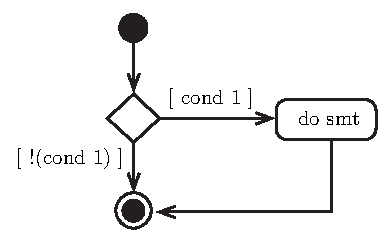
\includegraphics[width=0.50\linewidth]{01_Basics/figures/uml/SelectionStatement-00-UML-if-else.pdf}
\caption{UML \texttt{if-else} Activity Diagram Representation}
\label{fig:ch01_Basics_UML_SelStatement-00-if-else}
%~\ref{fig:ch01_Basics_UML_SelStatement-00-if-else} 
\end{figure}       %%%%%%%%%%%%%%%%%%%%%%% End Figure

\subsection{Iteration statement}
\subsubsection{\texttt{while}}
\begin{figure}[!h] %%%%%%%%%%%%%%%%%%%%%%% Begin Figure Directory
\centering
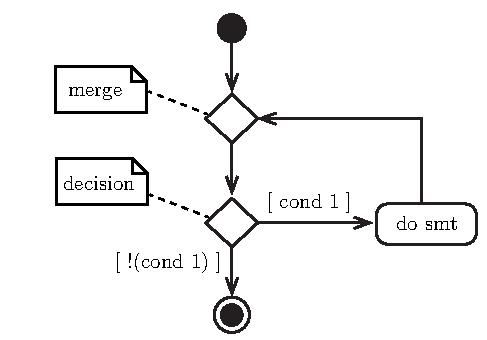
\includegraphics[width=0.50\linewidth]{01_Basics/figures/uml/IterationStatement-00-UML-while.pdf}
\caption{UML \texttt{if-else} Activity Diagram Representation}
\label{fig:ch01_Basics_UML_IterationStatement-00-while}
%~\ref{fig:ch01_Basics_UML_IterationStatement-00-while} 
\end{figure}       %%%%%%%%%%%%%%%%%%%%%%% End Figure



% no numbers listing
% \begin{lstlisting}[frame=tlrb,numbers=none,mathescape=true,escapechar=\%,columns=flexible]

% \begin{minipage}{.9\textwidth}
% \begin{lstlisting}[frame=tlrb,showlines=htrue,firstnumber=1,mathescape=true,escapechar=\%,columns=flexible]
% //code here
% \end{lstlisting}
% \end{minipage}

% \begin{lstlisting}[frame=tlrb,showlines=htrue,firstnumber=1,mathescape=true,escapechar=\%,columns=flexible]
% //Program 12.1
% \end{lstlisting}
    
%reference:
%~\ref{tab:t_ch11_UART_Registers} tab:t_ch12_edgeTriggeredModes
%~\ref{fig:RT_ch01} 
%\texttt{Ascii}
%\texttt{UART}
%\texttt{mailbox}
%\texttt{FIFO}
%\texttt{I/O}
%\underline{}
%$\texttt{b}_0$
%\sim = ~

%percent
%n%\%%10;

%for loops
% \newcounter{nnCount}
% \forloop{nnCount}{0}{\value{nnCount}<8}{&IME }  
% \forloop{nnCount}{0}{\value{nnCount}<8}{&PMC\arabic{nnCount} }


%Equation array
% \begin{eqnarray*}
%  & = & \text{minimun}\\
%  & = & \text{maximun}\\
%  & = &  \\
%  & = & \\
%  & = & 
% \end{eqnarray*}

% \begin{description}
% \item[Remark 1] If
% \end{description}

% \begin{description}
% \item[Remark 1] If
% \item[Remark 2] An
% \item[Remark 3] With 
% \end{description}

%Poner figura
% \begin{figure}[!h] %%%%%%%%%%%%%%%%%%%%%%% Begin Figure Directory
% \centering
% \includegraphics[width=0.70\linewidth]{figuresRT/ch06/RT-CH06-
% \caption{Free-space management.}
% \label{fig:ch01_00}
% %~\ref{ffig:ch01_00} 
% \end{figure}       %%%%%%%%%%%%%%%%%%%%%%% End Figure

%Poner Figura con minipages
% %begin minipages
% \begin{minipage}{.45\textwidth}
% %here some text.
% \end{minipage}
% \begin{minipage}{.55\textwidth}
% %and here the image.
% \centering
% \includegraphics[width=0.95\linewidth]{figures/ch12/ch12_lab12_squeme1.pdf}
% \captionof{figure}{Lab 12 diagram connections}
%\label{fig:RT_ch04_MACQ-EXAMPLE-01-oldDataIsLost}
%~\ref{fig:RT_ch04_MACQ-EXAMPLE-01-oldDataIsLost} 
% \end{minipage}
% \vspace{0.5cm}
% %end minipages


%\begin{enumerate}
%	\item Initialize timer and directions registers
%    \item Specify initial state
%    \item Perform FSM controller
%   \begin{enumerate}
%    	\item Call an output function, which depends on the state
%        \item Delay, which depends on the state
%        \item Call an input function to get the status of the coin sensors
%        \item Change states, which dependes on the state and the input
%    \end{enumerate}
%\end{enumerate}

% \begin{enumerate}
% 	\item Current instruction is finished,
%     \item Eight registers are pushed on the stack,
%     \item LR is set to 0xFFFFFFF9,
%     \item IPSR is set to the interrupt number,
%     \item PC is loaded with the interrupt vector
% \end{enumerate}

% Itemize categoriza poniendo (.) en lugar de números
% \begin{itemize} 
% 	\item I
% 	\item I
% 	\item Y
% 	\item Y
% 	\item Y
% 	\item Y
% 	\item 
% \end{itemize}

% \begin{table}[!h]
% \centering
% \begin{tabular}{|l|l|l|} \hline
% $p$ & bit Field & Interrupt         \\\hline
% $3$ & \bitsRange[31]{29} & Interrupt [$4m+3$]  \\\hline
% $2$ & \bitsRange[23]{21} & Interrupt [$4m+2$]  \\\hline
% $1$ & \bitsRange[15]{13} & Interrupt [$4m+1$]  \\\hline
% $0$ & \bitsRange[7]{5} & Interrupt [$4m$]   \\\hline
% \end{tabular}
% \caption{pasteCaption}
% \label{tab:t_rt_ch04_}
% ~\ref{tab:t_rt_ch04_}
% \end{table}

% Insertar URL
%\url{https://www.osha.gov/Publications/laboratory/OSHAfactsheet-laboratory-safety-noise.pdf}\\

% \newcommand{\bitsRange}[2][50]{\texttt{{#1}-{#2}}}
% \newcommand{\CustomHex}[2][0000]{\texttt{0x{#1}.{#2}}}
% \newcommand{\GPIOPort}[1]{\texttt{GPIO\_PORT{#1}}}
% \newcommand{\GPIOPortR}[2][A]{\texttt{GPIO\_PORT{#1}\_{#2}\_R}}
% \newcommand{\GPIOPortHandler}[1]{\texttt{GPIO\_PORT{#1}\_Handler}}
% \newcommand{\HandlerISR}[1]{\texttt{#1\_Handler}}
% \newcommand{\IRQnr}[1]{\texttt{{#1}}}
% \newcommand{\NVICPRI}[1]{\texttt{NVIC\_PRI{#1}\_R}}
% \newcommand{\NVICEN}[1]{\texttt{NVIC\_EN{#1}\_R}}
% \newcommand{\NVICDIS}[1]{\texttt{NVIC\_DIS{#1}\_R}}
% \newcommand{\Ttimer}[2][A]{\texttt{Timer\_{#2}{#1}}}
% \newcommand{\xNrbit}[1]{$#1$-\texttt{bit}}
% \newcommand{\xNrbits}[1]{$#1$-\texttt{bits}}
% \newcommand{\camouflagegreenCellColor}{\cellcolor[rgb]{0.47, 0.53, 0.42}}
% \newcommand{\lavenderCellColor}{\cellcolor[rgb]{0.9, 0.9, 0.98}}
% \newcommand{\volties}[2][0]{$\si{{#1}\volt}_{#2}$}
% \newcommand{\volti}[1]{$\si{{#1}\volt}$}
% \newcommand{\voltiposi}[1]{$+\si{{#1}\volt}$}
% \newcommand{\voltinega}[1]{$-\si{{#1}\volt}$}     \newpage
\section{Usefull Libraries}
\label{sec:Libraries}
%~\cref{sec:Libraries}
\subsection{\texttt{<cmath>}}

%%%%%%%%%%%%%%%%%%%%%%%%%%%%%%%%%%% CMATH TABLE
\begin{table}[!h]
\centering
\arrayrulecolor{black}
\begin{tabular}{l|l|l|l|} 
\cline{2-4}
 & Function & Description & Example \\ 
\hhline{>{\TabelleArrayColorGray}->{\arrayrulecolor{black}}---|}
\TabelleRowColorGray  01 & \texttt{ceil(x)} 
                         & rounds $x$ to the smallest integer not less than $x$ 
                         & \begin{tabular}[c]{@{}>{\TabelleRowCellGray}l@{}}
                         \texttt{ceil(9.2)} $=10.0$\\
                         \texttt{ceil(-9.8)} $=-9.0$\end{tabular} \\
02  & \texttt{cos(x)}  
    & trigonometric cosine of $x$ ($x$ in radians)  
    & $\texttt{cos(0.0)}=1.0$ \\
\TabelleRowColorGray 03 & \texttt{exp(x)} 
                        &  exponential function $e^{x}$
                        &  $\texttt{exp(1.0)} = 2.718282$\\
04  & \texttt{fabs(x)} 
    &  absolute value of $x$ 
    &   \begin{tabular}[c]{@{}l@{}}
        $\texttt{fabs(5.1)}=5.1$\\
        $\texttt{fabs(0.0)}=0.0$\\
        $\texttt{fabs(-8.6)}=8.6$\end{tabular} \\
\TabelleRowColorGray 05 & \texttt{floor(x)}  
                        &  rounds $x$ to the largest integer not greater than $x$
                        &  \begin{tabular}[c]{@{}>{\TabelleRowCellGray}l@{}}
                         \texttt{floor(9.2)} $=9.0$\\
                         \texttt{floor(-9.8)} $=-10$\end{tabular} \\
06  & \texttt{fmod(x, y)} 
    & remainder of $x/y$ as a floating-point number  
    & $\texttt{fmod(2.6, 1.2)}=0.2$ \\
\TabelleRowColorGray 07 & \texttt{log(x)} 
                        &  natural logarithm of $x$ (base $e$)
                        &  $\texttt{log()2.718282}=1.0$\\
08  & \texttt{log10(x)} 
    &  logarithm of $x$ (base 10)
    &  \begin{tabular}[c]{@{}l@{}}
        $\texttt{log10(10.0)}=1.0$\\
        $\texttt{log10(100.0)}=2.0$\end{tabular} \\
\TabelleRowColorGray 09 & \texttt{pow(x, y)} 
                        &  $x$ raised to power $y$, i.e. $x^y$
                        &  $\texttt{pow(2.7)}=2^{7}=128$\\
10  & \texttt{sin(x)} 
    &  trigonometric sine of x (x in radians)
    &  $\texttt{sin(0.0)}=0$\\
\TabelleRowColorGray 11 & \texttt{sqrt(x)} 
                        &  square root of x (where $x>=0$)
                        &  $\texttt{sin(9.0)}=3.0$\\
12  & \texttt{tan(x)} 
    &  trigonometric tangent of $x$ ($x$ in radians)
    &  $\texttt{tan(0.0)}=0$\\
\hhline{>{\TabelleArrayColorGray}->{\arrayrulecolor{black}}---|}
\end{tabular}
\end{table}

%%%%%%%% END CMATH TABLE






% \newcommand{\lavenderCellColor}{\cellcolor[rgb]{0.9, 0.9, 0.98}}
% \newcommand{\TabelleRowColorGray}{\rowcolor[rgb]{0.812,0.812,0.812}}
% \newcommand{\TabelleArrayColorGray}{\arrayrulecolor[rgb]{0.812,0.812,0.812}}
% \newcommand{\TabelleRowCellGray}{\cellcolor[rgb]{0.812,0.812,0.812}}
%

% no numbers listing
% \begin{lstlisting}[frame=tlrb,numbers=none,mathescape=true,escapechar=\%,columns=flexible]

% \begin{minipage}{.9\textwidth}
% \begin{lstlisting}[frame=tlrb,showlines=htrue,firstnumber=1,mathescape=true,escapechar=\%,columns=flexible]
% //code here
% \end{lstlisting}
% \end{minipage}

% \begin{lstlisting}[frame=tlrb,showlines=htrue,firstnumber=1,mathescape=true,escapechar=\%,columns=flexible]
% //Program 12.1
% \end{lstlisting}
    
%reference:
%~\ref{tab:t_ch11_UART_Registers} tab:t_ch12_edgeTriggeredModes
%~\ref{fig:RT_ch01} 
%\texttt{Ascii}
%\texttt{UART}
%\texttt{mailbox}
%\texttt{FIFO}
%\texttt{I/O}
%\underline{}
%$\texttt{b}_0$
%\sim = ~

%percent
%n%\%%10;

%for loops
% \newcounter{nnCount}
% \forloop{nnCount}{0}{\value{nnCount}<8}{&IME }  
% \forloop{nnCount}{0}{\value{nnCount}<8}{&PMC\arabic{nnCount} }


%Equation array
% \begin{eqnarray*}
%  & = & \text{minimun}\\
%  & = & \text{maximun}\\
%  & = &  \\
%  & = & \\
%  & = & 
% \end{eqnarray*}

% \begin{description}
% \item[Remark 1] If
% \end{description}

% \begin{description}
% \item[Remark 1] If
% \item[Remark 2] An
% \item[Remark 3] With 
% \end{description}

%Poner figura
% \begin{figure}[!h] %%%%%%%%%%%%%%%%%%%%%%% Begin Figure Directory
% \centering
% \includegraphics[width=0.70\linewidth]{figuresRT/ch06/RT-CH06-
% \caption{Free-space management.}
% \label{fig:ch01_00}
% %~\ref{ffig:ch01_00} 
% \end{figure}       %%%%%%%%%%%%%%%%%%%%%%% End Figure

%Poner Figura con minipages
% %begin minipages
% \begin{minipage}{.45\textwidth}
% %here some text.
% \end{minipage}
% \begin{minipage}{.55\textwidth}
% %and here the image.
% \centering
% \includegraphics[width=0.95\linewidth]{figures/ch12/ch12_lab12_squeme1.pdf}
% \captionof{figure}{Lab 12 diagram connections}
%\label{fig:RT_ch04_MACQ-EXAMPLE-01-oldDataIsLost}
%~\ref{fig:RT_ch04_MACQ-EXAMPLE-01-oldDataIsLost} 
% \end{minipage}
% \vspace{0.5cm}
% %end minipages

% %Poner Figura y al costado codigo
% %begin minipages
% \begin{minipage}{.60\textwidth}
% %%%%%%%%%%%%%%%%%%%%%%%%%%%%%%%%%Figure Selection Statement - while
% \centering
% 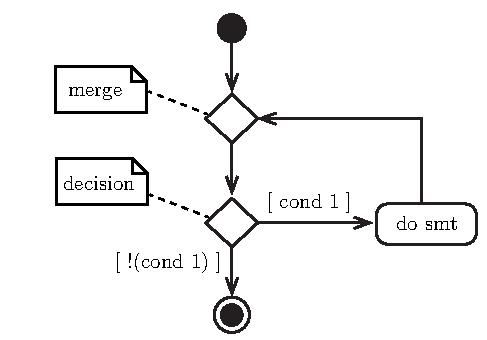
\includegraphics[width=0.50\linewidth]{01_Basics/figures/uml/IterationStatement-00-UML-while.pdf}
% \captionof{figure}{UML \texttt{while} Activity Diagram Representation}
% \label{fig:ch01_Basics_UML_IterationStatement-00-while}
% %~\ref{fig:ch01_Basics_UML_IterationStatement-00-while} 
% %%%%%%%%%%%%%%%%%%%%%%%%%%End figure
% \end{minipage}
% \begin{minipage}{.25\textwidth}
% %%%%%%%%%%%%%%%%%%%%%%%%%%%%%%%%%Begin code
% \begin{lstlisting}[frame=tlrb,numbers=none,mathescape=true,escapechar=\%,columns=flexible]
% some awesome code here
% \end{lstlisting}
% %%%%%%%%%%%%%%%%%%End Code
% \end{minipage}
% \vspace{0.5cm}
% %end minipages


%\begin{enumerate}
%	\item Initialize timer and directions registers
%    \item Specify initial state
%    \item Perform FSM controller
%   \begin{enumerate}
%    	\item Call an output function, which depends on the state
%        \item Delay, which depends on the state
%        \item Call an input function to get the status of the coin sensors
%        \item Change states, which dependes on the state and the input
%    \end{enumerate}
%\end{enumerate}

% \begin{enumerate}
% 	\item Current instruction is finished,
%     \item Eight registers are pushed on the stack,
%     \item LR is set to 0xFFFFFFF9,
%     \item IPSR is set to the interrupt number,
%     \item PC is loaded with the interrupt vector
% \end{enumerate}

% Itemize categoriza poniendo (.) en lugar de números
% \begin{itemize} 
% 	\item I
% 	\item I
% 	\item Y
% 	\item Y
% 	\item Y
% 	\item Y
% 	\item 
% \end{itemize}

% \begin{table}[!h]
% \centering
% \begin{tabular}{|l|l|l|} \hline
% $p$ & bit Field & Interrupt         \\\hline
% $3$ & \bitsRange[31]{29} & Interrupt [$4m+3$]  \\\hline
% $2$ & \bitsRange[23]{21} & Interrupt [$4m+2$]  \\\hline
% $1$ & \bitsRange[15]{13} & Interrupt [$4m+1$]  \\\hline
% $0$ & \bitsRange[7]{5} & Interrupt [$4m$]   \\\hline
% \end{tabular}
% \caption{pasteCaption}
% \label{tab:t_rt_ch04_}
% ~\ref{tab:t_rt_ch04_}
% \end{table}

% Insertar URL
%\url{https://www.osha.gov/Publications/laboratory/OSHAfactsheet-laboratory-safety-noise.pdf}\\

% \newcommand{\bitsRange}[2][50]{\texttt{{#1}-{#2}}}
% \newcommand{\CustomHex}[2][0000]{\texttt{0x{#1}.{#2}}}
% \newcommand{\GPIOPort}[1]{\texttt{GPIO\_PORT{#1}}}
% \newcommand{\GPIOPortR}[2][A]{\texttt{GPIO\_PORT{#1}\_{#2}\_R}}
% \newcommand{\GPIOPortHandler}[1]{\texttt{GPIO\_PORT{#1}\_Handler}}
% \newcommand{\HandlerISR}[1]{\texttt{#1\_Handler}}
% \newcommand{\IRQnr}[1]{\texttt{{#1}}}
% \newcommand{\NVICPRI}[1]{\texttt{NVIC\_PRI{#1}\_R}}
% \newcommand{\NVICEN}[1]{\texttt{NVIC\_EN{#1}\_R}}
% \newcommand{\NVICDIS}[1]{\texttt{NVIC\_DIS{#1}\_R}}
% \newcommand{\Ttimer}[2][A]{\texttt{Timer\_{#2}{#1}}}
% \newcommand{\xNrbit}[1]{$#1$-\texttt{bit}}
% \newcommand{\xNrbits}[1]{$#1$-\texttt{bits}}
% \newcommand{\camouflagegreenCellColor}{\cellcolor[rgb]{0.47, 0.53, 0.42}}
% \newcommand{\lavenderCellColor}{\cellcolor[rgb]{0.9, 0.9, 0.98}}
% \newcommand{\volties}[2][0]{$\si{{#1}\volt}_{#2}$}
% \newcommand{\volti}[1]{$\si{{#1}\volt}$}
% \newcommand{\voltiposi}[1]{$+\si{{#1}\volt}$}
% \newcommand{\voltinega}[1]{$-\si{{#1}\volt}$}              \newpage
\section{Arrays and Vectors}
\label{sec:Arrays-and-Vectors}
%~\cref{sec:Libraries}
\subsection{Difference}
\begin{itemize}
    \item \CppKeywordSpecial{array} - they are fixed-size collections consisting of data items of the same type
    \item \CppKeywordSpecial{vector} - same as array but they can grow and shrink dynamically at execution time. 
\end{itemize}

\subsection{Remarks}
\begin{itemize}
    \item When speaking about the elements of an array you could say:
\end{itemize}
\begin{table}[!h]
\centering
\begin{tblr}{
  row{3} = {c},
  row{4} = {c},
  cell{1}{1} = {c=3}{},
  cell{2}{1} = {c},
  cell{3}{1} = {r},
  cell{4}{1} = {r},
  hlines,
  vlines,
}
Example with an arrray declared as \texttt{arr}&  & \\
 & Refer to Subscript & Actual element in the array\\
"sevent element of the array" & \texttt{arr[6]} & 7\\
"array element 7"             & \texttt{arr[7]} & 8
\end{tblr}
\end{table}
\begin{itemize}
    \item Remeber \CppKeywordCommon{size\_t} := unsigned integral type. For more info see Section~\ref{subsec:Data-Type-Size-t}
\end{itemize}


\subsection{Array declaration}
%%%%%%%%%%%%%%%%%%%%%%%%%%%%%%%%%%%%%%%%%%%%%%%% Array Declaration
%\begin{minipage}{\MPWxCONSIDERxNUMERATIONxFORxLISTING\textwidth}
%\end{minipage}{\hspaceNumerationBeforeListing}
\begin{minipage}{\MPWxLARGExLISTING\textwidth} % = 0.8 times \textwidth
\vspaceTextToListing % =\vspace{0.1cm}
\begin{CPPCode}
array<type, arraySize> arrayName;
\end{CPPCode}
\end{minipage}
%%%%%%%%%%%%%%%%%%%%%%%% END Array Declaration
\\
Examples:\\
%%%%%%%%%%%%%%%%%%%%%%%%%%%%%%%%%%%%%%%%%%%%%%%% Array Declaration Examples
\begin{minipage}{\MPWxLARGExLISTING\textwidth} % = 0.8 times \textwidth
\vspaceTextToListing % =\vspace{0.1cm}
\begin{CPPCode}
array<int, 12> n1; ¿\hspace{3.2cm}¿// n1 is an array of 5 int values

array<int, 5> n2{32, 27, 64, 18, 95}; // ¿\codecomment{declaration and init}¿

array<int, 5> n3{}; ¿\hspace{3.0cm}¿// ¿\codecomment{initialize elements with 0}¿

//constant varaiable can be used to specify ¿\codecomment{array size}¿
const size_t arraySize{5} 
array<int, ¿arraySize¿> n4{10, 20, 30}; //values; 
\end{CPPCode}
\end{minipage}
\\
%%%%%%%%%%%%%%%%%%%%%%%% END Array Declaration examples
If there are fewer initializers than array elements, the remaining array elements are initialized
to zero.\\

\noindent Going through an array called \texttt{a}\\
%%%%%%%%%%%%%%%%%%%%%%%%%%%%%%%%%%%%%%%%%%%%%%%%% going through array
\begin{minipage}{\MPWxLARGExLISTING\textwidth} % = 0.8 times \textwidth
\vspaceTextToListing % =\vspace{0.1cm}
\begin{CPPCode}
for (size_t j{0}; j ¿<¿ a.size(); ++j)
{
    //¿\codecomment{do smt}¿
}
\end{CPPCode}
\end{minipage}
%%%%%%%%%%%%%%%%%%%%%%%% END going through array

\subsection{Array Declaration in range-Based style}
%%%%%%%%%%%%%%%%%%%%%%%%%%%%%%%%%%%%%%%%%%%%%%%%% 
\begin{minipage}{\MPWxXSSxLISTING\textwidth} % = 0.36 times \textwidth
\vspace{-0.35cm}
\vspaceTextToListing % =\vspace{0.1cm}
\begin{CPPCode}
//Range-based style
array<int, 5> items{1, 2, 3, 4, 5};
for (int item : items)
{
    cout ¿<¿¿<¿ item ¿<¿¿<¿ " ";
}
\end{CPPCode}
\end{minipage}
\hspaceListingToListing
\begin{minipage}{\MPWxXSxLISTING\textwidth} % = 0.8 times \textwidth
\vspaceTextToListing % =\vspace{0.1cm}
\begin{CPPCode}
//Equivalent to:
for ( int counter{0}; 
             counter ¿<¿ items.size(); 
          ++counter )
{
    cout ¿<¿¿<¿ items[counter] ¿<¿¿<¿ " ";
}
\end{CPPCode}
\end{minipage}
\\
%%%
\noindent To modify the elements we need the ampersand symbol \texttt{\&}, i.e.:\\
%%%%%%%%%%%%%%%%%%%%%%%%%%%%%%%%%%%%%%%%%%%%%%%%% 
\begin{minipage}{\MPWxLARGExLISTING\textwidth} % = 0.8 times \textwidth
\vspaceTextToListing % =\vspace{0.1cm}
\begin{CPPCode}
for (int& itemRef : items)
{
    itemRef *= 2;    // ¿\codecomment{do smt modifying the content}¿
}
\end{CPPCode}
\end{minipage}

\subsection{Multidimensional array}
\begin{minipage}{\MPWxSMALLxLISTING\textwidth} % = 0.8 times \textwidth
\vspaceTextToListing % =\vspace{0.1cm}
\begin{CPPCode}
#include <iostream>
#include <array>
/* GLOBALS VARIABLES*/
const size_t rows{2};
const size_t columns{3};

/* PROTOTYPES */
void printArray(const array<array<int, columns>, rows>&);
\end{CPPCode}
\end{minipage}
\hspaceListingToListing
\begin{minipage}{\MPWxXXSxLISTING\textwidth} % = 0.8 times \textwidth
Note that \CppKeywordCommon{const} is used in the function prototype since we are not changing the values. Meanwhile \CppKeywordCommon{const}\texttt{\&} in the row's declaration indicates that the reference \textbf{cannot} be used to \textbf{modify} the rows and prevents each row from being copied into the range variable.
\end{minipage}
\\
\begin{minipage}{\MPWxSMALLxLISTING\textwidth} % = 0.8 times \textwidth
\vspaceTextToListing % =\vspace{0.1cm}
\begin{CPPCode}
int main()
{
    array<array<int, columns>, rows> array1{1, 2, 3, 4, 5, 6};
    array<array<int, columns>, rows> array2{1, 2, 3, 4, 5};

    cout ¿<¿¿<¿ "Values ¿in¿ array1 by row are:" ¿<¿¿<¿ endl;
    printArray(array1);

    cout ¿<¿¿<¿ "\nValues ¿in¿ array2 by row are:" ¿<¿¿<¿ endl;
    printArray(array2);
}

void printArray(const array<array<int, columns>, rows>& a)
{
    for (auto const& row : a)
    {
        for (auto const& element : row)
        {
            cout ¿<¿¿<¿ element ¿<¿¿<¿ ' ';            
        }

        cout ¿<¿¿<¿ endl;
    }
}
\end{CPPCode}
\end{minipage}
\hspaceListingToListing
\begin{minipage}{\MPWxXXSxLISTING\textwidth} % = 0.8 times \textwidth
\vspace{5cm}
\vspaceTextToListing % =\vspace{0.1cm}
\begin{Terminal}
OUTPUT:
-----------------------------
Values in array1 by row are:
1 2 3
4 5 6

Values in array2 by row are:
1 2 3
4 5 0
\end{Terminal}
\end{minipage}\\
As an example, the next Listing present the multidimensional nested counter-controlled statement\\
\begin{minipage}{\MPWxSMALLxLISTING\textwidth} % = 0.8 times \textwidth
\vspaceTextToListing % =\vspace{0.1cm}
\begin{CPPCode}
for (size_t row{0}; row ¿<¿ a.size(); ++row)
{
    for (size_t column{0}; column ¿<¿ a[row].size(); ++column) 
    {
        cout ¿<¿¿<¿ a[row][column] ¿<¿¿<¿ ' ';
    }
    
    cout ¿<¿¿<¿ endl;
}
\end{CPPCode}
\end{minipage}

\subsection{Local Arrays}
A static local variable in a function definition exists for the program’s duration but is visible only in the function’s body.
\subsubsection{\CppKeywordCommon{static} local Array}
By declaring a local array as \CppKeywordCommon{static}, then it is not created and initialized each time the program calls the function and is not destroyed each time the function terminates. This can improve performance especially when using large arrays~\cite{deitel2017c++}.\\

\noindent If a static array is not initialized explicitly by you, \textbf{each element of that array is initialized to zero by the compiler} when the array is created. Recall that C++ does not perform such default initialization for other local variables.\\
\noindent
\begin{minipage}{\MPWxXSxLISTING\textwidth} % = 0.7 times \textwidth
\vspaceTextToListing % =\vspace{0.1cm}
        \begin{CPPCode}
const size_t arraySize{3};
void SomeFunction(void)
{
    // Local ¿\codecomment{array}¿
    array<int, arraySize> arr{1, 2, 3}
}
        \end{CPPCode}
    \end{minipage}
    \hspaceListingXSToListingXS
    \begin{minipage}{\MPWxSxLISTING\textwidth} % = 0.7 times \textwidth
    \vspaceTextToListing
        \begin{CPPCode}
const size_t arraySize{3};
void SomeFunction(void)
{
        // Static local ¿\codecomment{array}¿
    static array<int, arraySize> arrAsStaticLocal
}
        \end{CPPCode}
\end{minipage}

\subsection{Built-In Arrays}
\label{subsec:Built-In-Arrays}
%~\cref{subsec:Built-In-Arrays}
It is a fixed-size data structure. The compiler reserves the appropiate amount of memory. Its declaration goes as follows:
\codeLine{type arrayName[arraySize]}\\
where \CppCommonCode{arraySize}$>0$ and must be integer constant.\\
\begin{minipage}{\MPWxXSxLISTING\textwidth} % = 0.7 times \textwidth
\vspaceTextToListing % =\vspace{0.1cm}
        \begin{CPPCode}
//init opt 01
int n[5]{50, 20, 30, 10, 40}
        \end{CPPCode}
    \end{minipage}
    \hspaceListingXSToListingXS
    \begin{minipage}{\MPWxSxLISTING\textwidth} % = 0.7 times \textwidth
    \vspaceTextToListing
        \begin{CPPCode}
//init opt 02  - possible but not recommended
int n[]{50, 20, 30, 10, 40} //arrSize no specified.
        \end{CPPCode}
\end{minipage}
\begin{itemize}
    \item if you provide fewer initializers than number of elements, the remaining elements are value initialized, i.e.
    \begin{itemize}
        \item numeric types to $0$, 
        \item \CppCommonCode{bool}s to false,
        \item \textbf{pointers} to \CppCommonCode{nullptr} (Pointers are explained in Section~\ref{sec:Pointers}) and 
        \item class objects to its default constructor.
    \end{itemize}

    \item built-in arrays don't know their own size, so a function that processes a built-in array should also have a parameter to receive its size.

    \item The compiler does not distinguish between a function that receives a pointer and a function that receives a built in array. I.e. each time that the compiler finds a built-in array notation it converts to pointer  notation.\\
    \begin{minipage}{\MPWxXXSxLISTING\textwidth} % = 0.7 times \textwidth
\vspaceTextToListing % =\vspace{0.1cm}
        \begin{CPPCode}
// Built-in Array notation
foo(const int values[])
        \end{CPPCode}
    \end{minipage}
    \hspaceListingXSToListingXS
    \begin{minipage}{\MPWxXSxLISTING\textwidth} % = 0.7 times \textwidth
    \vspaceTextToListing
        \begin{CPPCode}
// Pointer notation
foo(const int* values)
        \end{CPPCode}
\end{minipage}
    \item Note that \CppCommonCode{const int* values} is read as "values is a pointer to a integer constant".
\end{itemize}

\subsection{Examples}

\begin{minipage}{\MPWxLARGExLISTING\textwidth} % = 0.8 times \textwidth
\vspaceTextToListing % =\vspace{0.1cm}
\begin{CPPCode}
//example printArray
// output ¿\codecomment{array with two rows and three columns}¿
void printArray(const array<array<int, columns>, row>& row_x)
{
    // loop through ¿\codecomment{array}'¿s rows
    for (auto const& row : row_x)
    {
        // loop through columns of current row
        for (auto const& col : row)
        {
            cout ¿<¿¿<¿ element ¿<¿¿<¿ ' ';
        }
    }
}
\end{CPPCode}
\end{minipage}
\\
which is equivalent to:\\
\begin{minipage}{\MPWxLARGExLISTING\textwidth} % = 0.8 times \textwidth
\vspaceTextToListing % =\vspace{0.1cm}
\begin{CPPCode}
for (size_t row{0}; row ¿<¿ a.size(); ++row) 
{
    for (size_t column{0}; column ¿<¿ a[row].size(); ++column)
    {
        cout ¿<¿¿<¿ a[row][column] ¿<¿¿<¿ ' ';
    }
    cout ¿<¿¿<¿ endl;
}
\end{CPPCode}
\end{minipage}
\\

%%%%%%%%%%%%%%%%%%%%%%%% END going through array
% no numbers listing
% \begin{lstlisting}[frame=tlrb,numbers=none,mathescape=true,escapechar=\%,columns=flexible]

% \begin{minipage}{.9\textwidth}
% \begin{lstlisting}[frame=tlrb,showlines=htrue,firstnumber=1,mathescape=true,escapechar=\%,columns=flexible]
% //code here
% \end{lstlisting}
% \end{minipage}

% \begin{lstlisting}[frame=tlrb,showlines=htrue,firstnumber=1,mathescape=true,escapechar=\%,columns=flexible]
% //Program 12.1
% \end{lstlisting}
    
%reference:
%~\ref{tab:t_ch11_UART_Registers} tab:t_ch12_edgeTriggeredModes
%~\ref{fig:RT_ch01} 
%\texttt{Ascii}
%\texttt{UART}
%\texttt{mailbox}
%\texttt{FIFO}
%\texttt{I/O}
%\underline{}
%$\texttt{b}_0$
%\sim = ~

%percent
%n%\%%10;

%for loops
% \newcounter{nnCount}
% \forloop{nnCount}{0}{\value{nnCount}<8}{&IME }  
% \forloop{nnCount}{0}{\value{nnCount}<8}{&PMC\arabic{nnCount} }


%Equation array
% \begin{eqnarray*}
%  & = & \text{minimun}\\
%  & = & \text{maximun}\\
%  & = &  \\
%  & = & \\
%  & = & 
% \end{eqnarray*}

% \begin{description}
% \item[Remark 1] If
% \end{description}

% \begin{description}
% \item[Remark 1] If
% \item[Remark 2] An
% \item[Remark 3] With 
% \end{description}

%Poner figura
% \begin{figure}[!h] %%%%%%%%%%%%%%%%%%%%%%% Begin Figure Directory
% \centering
% \includegraphics[width=0.70\linewidth]{figuresRT/ch06/RT-CH06-
% \caption{Free-space management.}
% \label{fig:ch01_00}
% %~\ref{ffig:ch01_00} 
% \end{figure}       %%%%%%%%%%%%%%%%%%%%%%% End Figure

%Poner Figura con minipages
% %begin minipages
% \begin{minipage}{.45\textwidth}
% %here some text.
% \end{minipage}
% \begin{minipage}{.55\textwidth}
% %and here the image.
% \centering
% \includegraphics[width=0.95\linewidth]{figures/ch12/ch12_lab12_squeme1.pdf}
% \captionof{figure}{Lab 12 diagram connections}
%\label{fig:RT_ch04_MACQ-EXAMPLE-01-oldDataIsLost}
%~\ref{fig:RT_ch04_MACQ-EXAMPLE-01-oldDataIsLost} 
% \end{minipage}
% \vspace{0.5cm}
% %end minipages

% %Poner Figura y al costado codigo
% %begin minipages
% \begin{minipage}{.60\textwidth}
% %%%%%%%%%%%%%%%%%%%%%%%%%%%%%%%%%Figure Selection Statement - while
% \centering
% 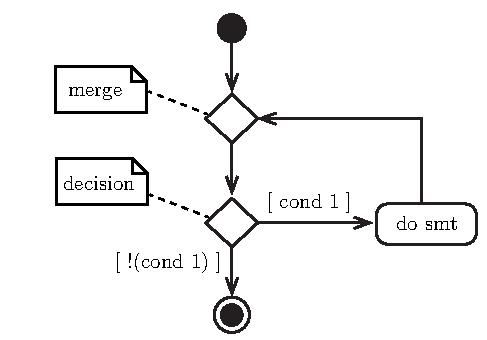
\includegraphics[width=0.50\linewidth]{01_Basics/figures/uml/IterationStatement-00-UML-while.pdf}
% \captionof{figure}{UML \texttt{while} Activity Diagram Representation}
% \label{fig:ch01_Basics_UML_IterationStatement-00-while}
% %~\ref{fig:ch01_Basics_UML_IterationStatement-00-while} 
% %%%%%%%%%%%%%%%%%%%%%%%%%%End figure
% \end{minipage}
% \begin{minipage}{.25\textwidth}
% %%%%%%%%%%%%%%%%%%%%%%%%%%%%%%%%%Begin code
% \begin{lstlisting}[frame=tlrb,numbers=none,mathescape=true,escapechar=\%,columns=flexible]
% some awesome code here
% \end{lstlisting}
% %%%%%%%%%%%%%%%%%%End Code
% \end{minipage}
% \vspace{0.5cm}
% %end minipages


%\begin{enumerate}
%	\item Initialize timer and directions registers
%    \item Specify initial state
%    \item Perform FSM controller
%   \begin{enumerate}
%    	\item Call an output function, which depends on the state
%        \item Delay, which depends on the state
%        \item Call an input function to get the status of the coin sensors
%        \item Change states, which dependes on the state and the input
%    \end{enumerate}
%\end{enumerate}

% \begin{enumerate}
% 	\item Current instruction is finished,
%     \item Eight registers are pushed on the stack,
%     \item LR is set to 0xFFFFFFF9,
%     \item IPSR is set to the interrupt number,
%     \item PC is loaded with the interrupt vector
% \end{enumerate}

% Itemize categoriza poniendo (.) en lugar de números
% \begin{itemize} 
% 	\item I
% 	\item I
% 	\item Y
% 	\item Y
% 	\item Y
% 	\item Y
% 	\item 
% \end{itemize}

% \begin{table}[!h]
% \centering
% \begin{tabular}{|l|l|l|} \hline
% $p$ & bit Field & Interrupt         \\\hline
% $3$ & \bitsRange[31]{29} & Interrupt [$4m+3$]  \\\hline
% $2$ & \bitsRange[23]{21} & Interrupt [$4m+2$]  \\\hline
% $1$ & \bitsRange[15]{13} & Interrupt [$4m+1$]  \\\hline
% $0$ & \bitsRange[7]{5} & Interrupt [$4m$]   \\\hline
% \end{tabular}
% \caption{pasteCaption}
% \label{tab:t_rt_ch04_}
% ~\ref{tab:t_rt_ch04_}
% \end{table}

% Insertar URL
%\url{https://www.osha.gov/Publications/laboratory/OSHAfactsheet-laboratory-safety-noise.pdf}\\

% \newcommand{\bitsRange}[2][50]{\texttt{{#1}-{#2}}}
% \newcommand{\CustomHex}[2][0000]{\texttt{0x{#1}.{#2}}}
% \newcommand{\GPIOPort}[1]{\texttt{GPIO\_PORT{#1}}}
% \newcommand{\GPIOPortR}[2][A]{\texttt{GPIO\_PORT{#1}\_{#2}\_R}}
% \newcommand{\GPIOPortHandler}[1]{\texttt{GPIO\_PORT{#1}\_Handler}}
% \newcommand{\HandlerISR}[1]{\texttt{#1\_Handler}}
% \newcommand{\IRQnr}[1]{\texttt{{#1}}}
% \newcommand{\NVICPRI}[1]{\texttt{NVIC\_PRI{#1}\_R}}
% \newcommand{\NVICEN}[1]{\texttt{NVIC\_EN{#1}\_R}}
% \newcommand{\NVICDIS}[1]{\texttt{NVIC\_DIS{#1}\_R}}
% \newcommand{\Ttimer}[2][A]{\texttt{Timer\_{#2}{#1}}}
% \newcommand{\xNrbit}[1]{$#1$-\texttt{bit}}
% \newcommand{\xNrbits}[1]{$#1$-\texttt{bits}}
% \newcommand{\camouflagegreenCellColor}{\cellcolor[rgb]{0.47, 0.53, 0.42}}
% \newcommand{\lavenderCellColor}{\cellcolor[rgb]{0.9, 0.9, 0.98}}
% \newcommand{\volties}[2][0]{$\si{{#1}\volt}_{#2}$}
% \newcommand{\volti}[1]{$\si{{#1}\volt}$}
% \newcommand{\voltiposi}[1]{$+\si{{#1}\volt}$}
% \newcommand{\voltinega}[1]{$-\si{{#1}\volt}$}     \newpage
\section{Passing Arguments with Pointers}
\label{sec:Passing Arguments with Pointers}
%~\cref{sec:Libraries}
There are three forms of passing arguments with pointers
\begin{itemize}
    \item Passing by value
    \item Passing by reference with a reference argument
    \item Passing by reference with a pointer argument
\end{itemize}       \newpage
\section{Including the class header in the source code file}
Example of using header (\texttt{.h}) and and the \texttt{.cpp} file\\
\begin{itemize}
    \item Inside the header we will define the class declaration.
    \item Mainwhile in the \texttt{.cpp} we will define the class-member functions.
\end{itemize}

\subsection{Header \texttt{.h}}
\begin{minipage}{\MPWxLARGExLISTING\textwidth} % = 0.8 times \textwidth
\vspaceTextToListing % =\vspace{0.1cm}
\begin{CPPCode}
#include <string.h>

//prevent multiple inclussion of header
#ifndef DATE_H
#define DATE_H

class Date{
public:
    explicit Date(unsigned int = 1, unsigned int = 1, unsigned int = 2000)
    std::string toString() const;
    
private:
    unsigned int moth;
    unsigned int day;
    unsigned int year;
}; //¿$\leftarrow$ \codecomment{do not}¿ forget the semicolon

#endif
\end{CPPCode}
\end{minipage}

\subsection{\texttt{.cpp}}
\begin{minipage}{\MPWxLARGExLISTING\textwidth} % = 0.8 times \textwidth
\vspaceTextToListing % =\vspace{0.1cm}
\begin{CPPCode}
#include <¿s¿tring> // ¿\codecomment{for ostringstream class}¿
#include <sstream>
#include <Date.h>   //INCLUDE DEFINITION OF THE HEADER!
using namespace std;

//Date constructor (should do range checking)
Date::Date(unsigned int m, unsigned d unsigned int y)
    : month{m}, day{d}, year{y} {}
    
//print Date in the format mm/dd/yyyy
string Date::toString() const {
    ostringstream output;
    output ¿<¿¿<¿ month ¿<¿¿<¿ '/' ¿<¿¿<¿ day ¿<¿¿<¿ '/' ¿<¿¿<¿ year;
    return output.str();
}
#endif
\end{CPPCode}
\end{minipage}

\newpage
\subsection{Example}
\begin{minipage}{\MPWxLARGExLISTING\textwidth} % = 0.8 times \textwidth
\vspaceTextToListing % =\vspace{0.1cm}
\begin{CPPCode}
#include <iostream>
#include "Date.h" // include definition of ¿\codecomment{class}¿ Date from Date.h
using namespace std;

int main()
{
    Date date1{7, 4, 2004};
    Date date2; // date2 defaults to 1/1/2000
    
    cout ¿<¿¿<¿ "date1 = " ¿<¿¿<¿ date1.toString() ¿<¿¿<¿ "\ndate2 = " ¿<¿¿<¿ date2.toString() ¿<¿¿<¿ "\n\n";
    
    cout ¿<¿¿<¿ "After default memberwise assignment, date2 = " ¿<¿¿<¿ date2.toString() ¿<¿¿<¿ endl;
}
\end{CPPCode}
\end{minipage}\\

\noindent{}
\begin{minipage}{\MPWxLARGExLISTING\textwidth} % = 0.8 times \textwidth
\vspaceTextToListing % =\vspace{0.1cm}
Output:\\
\vspace{-0.5cm}
\begin{Terminal}
date1 = 7/4/2004
date2 = 1/1/2000
After default memberwise assignment, date2 = 7/4/2004
\end{Terminal}
\end{minipage}                 \newpage
\section{Usefull keyword and concepts remarks}
\label{sec:Useufull-keyword-remarks}
%~\cref{sec:Useufull-keyword-remarks}
\subsection{Predicate and utility functions}
\label{subsec:Keyword auto}
%~\cref{subsec:Useufull-keyword-remarks-00-fcn-predicate-utility}
A \textbf{predicate function} (also known as \textbf{access function}) are basically functions that can read or display data. Also functions thatn can be read and serves to test the truth or falsity of conditions.\\

\noindent A \textbf{utility function} (also known as helper function) is a \CppKeywordCommon{private} member function that supports the operation of the class\textquotesingle{}\,s \CppKeywordCommon{public} member functions, but is \underline{not} intended for use by clients of the class


\subsection{Keyword \texttt{auto}}
\label{subsec:Keyword auto}
%~\cref{subsec:Useufull-keyword-remarks-01-Keyword-auto}
One of the most important advantage of using \CppKeywordCommon{auto} is that you need to initialize the variable. Normally you can track your type and also deduce your type. 
\begin{itemize}
    %%%%%%%%%%%%%%%%%%%%%%%%%%%%%%%%%%%%%%%%%% ITEM 
    \item To make th type track, deduce:\\
    \begin{minipage}{\MPWxXXSxLISTING\textwidth} % = 0.7 times \textwidth
    \vspaceTextToListing % =\vspace{0.1cm}
        \begin{CPPCode}
auto var = init;
        \end{CPPCode}
    \end{minipage}\\ 
    Example given:\\
\begin{minipage}{\MPWxXXSxLISTING\textwidth} % = 0.7 times \textwidth
\vspaceTextToListing % =\vspace{0.1cm}
        \begin{CPPCode}
//old style:
const char* s = "Hello";
widget w = get_widget();
        \end{CPPCode}
    \end{minipage}
    \hspaceListingXSToListingXS
    \begin{minipage}{\MPWxXXSxLISTING\textwidth} % = 0.7 times \textwidth
    \vspaceTextToListing
        \begin{CPPCode}
//better style:
auto s = "Hello";
auto w = get_widget();
        \end{CPPCode}
    \end{minipage}
    %%%%%%%%%%%%%%%%%%%%%%%%%%%%%%%%%%%%%%%%%% ITEM 
    \item To make type stick, commit:\\
    \begin{minipage}{\MPWxXXSxLISTING\textwidth} % = 0.7 times \textwidth
\vspaceTextToListing % =\vspace{0.1cm}
        \begin{CPPCode}
        auto var = type{ init };
\end{CPPCode}
\end{minipage}\\
 \begin{minipage}{\MPWxXXSxLISTING\textwidth} % = 0.7 times \textwidth
\vspaceTextToListing % =\vspace{0.1cm}
\begin{CPPCode}
        type var{ init };
\end{CPPCode}
    \end{minipage}\\
    Example given:\\
\begin{minipage}{\MPWxXXSxLISTING\textwidth} % = 0.7 times \textwidth
\vspaceTextToListing % =\vspace{0.1cm}
        \begin{CPPCode}
//old style:
employee e{ empid };
widget w{ 12, 34};
        \end{CPPCode}
    \end{minipage}
    \hspaceListingXSToListingXS
    \begin{minipage}{\MPWxXXSxLISTING\textwidth} % = 0.7 times \textwidth
    \vspaceTextToListing
        \begin{CPPCode}
//better style:
auto e = employee{ empid };
auto w = widget{ 12, 34};
        \end{CPPCode}
    \end{minipage}
    
    %%%%%%%%%%%%%%%%%%%%%%%%%%%%%%%%%%%%%%%%%% ITEM 
    \item With heap allocation, type is on the right naturally anyway\\
    \begin{minipage}{\MPWxXXSxLISTING\textwidth} % = 0.7 times \textwidth
\vspaceTextToListing % =\vspace{0.1cm}
        \begin{CPPCode}
auto w = new widget{}           
auto w = make_unique<widget>();
        \end{CPPCode}
    \end{minipage}
    \hspaceListingXSToListingXS
    \begin{minipage}{\MPWxXXSxLISTING\textwidth} % = 0.7 times \textwidth
    \vspaceTextToListing
        \begin{CPPCode}
C++98 Style
C++14 Style
        \end{CPPCode}
    \end{minipage}

    %%%%%%%%%%%%%%%%%%%%%%%%%%%%%%%%%%%%%%%%%% ITEM 
    \item However, what about \CppKeywordCommon{int} vs \CppKeywordCommon{auto} ?\\
        \begin{minipage}{\MPWxXXSxLISTING\textwidth} % = 0.7 times \textwidth
\vspaceTextToListing % =\vspace{0.1cm}
        \begin{CPPCode}
int x = 42;
        \end{CPPCode}
    \end{minipage}
    \hspaceListingXSToListingXS
    \begin{minipage}{\MPWxXXSxLISTING\textwidth} % = 0.7 times \textwidth
    \vspaceTextToListing
        \begin{CPPCode}
auto = 42;
        \end{CPPCode}
    \end{minipage}

    %%%%%%%%%%%%%%%%%%%%%%%%%%%%%%%%%%%%%%%%%% ITEM 
    \item Well there are two arguments: consistency, and no narrowing. Additionally, you can use literal suffixes\\
    \begin{minipage}{\MPWxXXSxLISTING\textwidth} % = 0.7 times \textwidth
\vspaceTextToListing % =\vspace{0.1cm}
        \begin{CPPCode}
employee e{ empid };
widget w{ 12, 34};
int x = 42;
float x = 42;
unsigned long x = 42;
string x = "42";
chrono::nanoseconds x{42}
        \end{CPPCode}
    \end{minipage}
    \hspaceListingXSToListingXS
    \begin{minipage}{\MPWxXXSxLISTING\textwidth} % = 0.7 times \textwidth
    \vspaceTextToListing
        \begin{CPPCode}
auto e = employee{ empid };
auto w = widget{ 12, 34};
auto x = 42;
auto x = 42.f;       //lit. suffix
auto x = 42.ul; //lit. suffix
auto x = "42"s  //C++14
auto x = 42ns       //C++14
        \end{CPPCode}
    \end{minipage}

    %%%%%%%%%%%%%%%%%%%%%%%%%%%%%%%%%%%%%%%%%% ITEM 
    \item In function declaration and named lambdas( 1st and 2nd row respec.):\\
    \begin{minipage}{\MPWxXXSxLISTING\textwidth} % = 0.7 times \textwidth
\vspaceTextToListing % =\vspace{0.1cm}
        \begin{CPPCode}
int f( double )

        \end{CPPCode}
    \end{minipage}
    \hspaceListingXSToListingXS
    \begin{minipage}{\MPWxXXSxLISTING\textwidth} % = 0.7 times \textwidth
    \vspaceTextToListing
        \begin{CPPCode}
auto f (double) -> int;
auto f = [=](double) { /*... */ }
        \end{CPPCode}
    \end{minipage}

    %%%%%%%%%%%%%%%%%%%%%%%%%%%%%%%%%%%%%%%%%% ITEM 
    \item Aliases (no more typedefs)\\
    \begin{minipage}{\MPWxXXSxLISTING\textwidth} % = 0.7 times \textwidth
\vspaceTextToListing % =\vspace{0.1cm}
        \begin{CPPCode}
typedef set<string>dict;
        \end{CPPCode}
    \end{minipage}
    \hspaceListingXSToListingXS
    \begin{minipage}{\MPWxXXSxLISTING\textwidth} % = 0.7 times \textwidth
    \vspaceTextToListing
        \begin{CPPCode}
using dict = set<string>;
        \end{CPPCode}
    \end{minipage}

    %%%%%%%%%%%%%%%%%%%%%%%%%%%%%%%%%%%%%%%%%% ITEM 
    \item Template aliases\\
    \begin{minipage}{\MPWxXXSxLISTING\textwidth} % = 0.7 times \textwidth
\vspaceTextToListing % =\vspace{0.1cm}
        \begin{CPPCode}
template<class T>struct myvec
{typedef vector<T,myalloc> type;}
        \end{CPPCode}
    \end{minipage}
    \hspaceListingXSToListingXS
    \begin{minipage}{\MPWxXXSxLISTING\textwidth} % = 0.7 times \textwidth
    \vspaceTextToListing
        \begin{CPPCode}
template<class T>
using myvec = vector<T,myalloc>;
        \end{CPPCode}
    \end{minipage}
\end{itemize}
%%%%%%%%%%%%%%%%%%%%%%%%%% END ITEMIZE
\newpage
\noindent Here a few more examples:\\
\begin{itemize}
    %%%%%%%%%%%%%%%%%%%%%%%%%%%%%%%%%%%%%%%%%% ITEM 
    \item  Example 01: altough is modern code people kept not noticing the different types\\
    \begin{minipage}{\MPWxXXSxLISTING\textwidth} % = 0.7 times \textwidth
\vspaceTextToListing % =\vspace{0.1cm}
        \begin{CPPCode}
base* pb = new derived()
        \end{CPPCode}
    \end{minipage}
    \hspaceListingXSToListingXS
    \begin{minipage}{\MPWxSxLISTING\textwidth} % = 0.5 times \textwidth
    \vspaceTextToListing
        \begin{CPPCode}
unique_ptr<base> pb = make_unique<derived>()
        \end{CPPCode}
    \end{minipage}

    %%%%%%%%%%%%%%%%%%%%%%%%%%%%%%%%%%%%%%%%%% ITEM 
    \item  Example 02: altough is modern code people kept not noticing the different types\\
    \begin{minipage}{\MPWxXXSxLISTING\textwidth} % = 0.7 times \textwidth
\vspaceTextToListing % =\vspace{0.1cm}
        \begin{CPPCode}
base* pb = new derived()
        \end{CPPCode}
    \end{minipage}
    \hspaceListingXSToListingXS
    \begin{minipage}{\MPWxSxLISTING\textwidth} % = 0.5 times \textwidth
    \vspaceTextToListing
        \begin{CPPCode}
auto pb = make_unique<base>{ make_unique<derived>() }
        \end{CPPCode}
    \end{minipage}
\end{itemize}

\noindent For cases where you can't use \CppKeywordCommon{auto} please see min 47:35 in \href{https://www.youtube.com/watch?v=xnqTKD8uD64}{CppCon 2014: Back to the basics! Essentials of Modern C++ Style}


\subsection{Scope Operator \texttt{::}}
\label{subsec:Useufull-keyword-remarks-02-Unary-Operator}
%~\cref{subsec:Useufull-keyword-remarks-02-Unary-Operator}
Also known as unary Scope resolution operator (::). It provides access to a global variable when is ambiguous to which variable refers. The latter is normally caused due to a duplicate name of a variable in scope. E.g.:\\
\begin{minipage}{\MPWxLARGExLISTING\textwidth} % = 0.8 times \textwidth
\vspaceTextToListing % =\vspace{0.1cm}
\begin{CPPCode}
#include <iostream>
using namespace std;

int number{7};

int main()
{
    double number{10.5};
    cout ¿<¿¿<¿ "¿Local double value of number¿ = " ¿<¿¿<¿ number
           ¿<¿¿<¿ ¿"\textbackslash{}nGlobal int value of number¿ = " ¿<¿¿<¿ ::number ¿<¿¿<¿ endl;
}
\end{CPPCode}
\end{minipage}\\
\begin{minipage}{\MPWxLARGExLISTING\textwidth} % = 0.8 times \textwidth
\vspaceTextToListing % =\vspace{0.1cm}
\vspace{-0.3cm}
\begin{Terminal}
Local double value of number = 10.5
Global int value of number = 7 ¿\hspace{2cm}$\leftarrow$ used with the Scope Operator¿
\end{Terminal}
\end{minipage}
%\noindent 

\subsection{Function Template}
\label{subsec:Useufull-keyword-remarks-03-Function-Template}
%~\cref{subsec:Useufull-keyword-remarks-03-Function-Template}
C++ provides a compact way to define overloaded functions by means of Function templates, which generates separate function templates specializations to handle each type call appropiately.\\
\begin{minipage}{\MPWxLARGExLISTING\textwidth} % = 0.8 times \textwidth
\vspaceTextToListing % =\vspace{0.1cm}
\begin{CPPCode}
// The header, e.g. maximum.h
template <typename T>                       // also possible¿\codecomment{: template<class T>}¿
T maximum(T val01, T val02, T val03)
{
    return (val03 > val02) 
                ? ( ( val03 > val01 ) ? val03 : val01 )
                : ( ( val02 > val01 ) ? val02 : val01 )
}
\end{CPPCode}
\begin{CPPCode}
// The cpp program, e.g. Test_maximum.cpp
#include <iostream>
#include "maximum.h"
using namespace std;

int main()
{
    auto int1{1},int2{2},int3{3};
    auto double1{3.3},double2{1.1},double3{2.2};
    auto char1{'A'},char2{'C'},char3{'B'};

    cout ¿<¿¿<¿ "The maximum integer value is: "
           ¿<¿¿<¿ maximum(int1,int2,int3);

    cout ¿<¿¿<¿ "\nThe maximum double value is: "
           ¿<¿¿<¿ maximum(double1,double2,double3);

    cout ¿<¿¿<¿ "\nThe maximum character value is: "
           ¿<¿¿<¿ maximum(char1,char2,char3);
}
\end{CPPCode}
\end{minipage}\\
\begin{minipage}{\MPWxLARGExLISTING\textwidth} % = 0.8 times \textwidth
\vspaceTextToListing % =\vspace{0.1cm}
\vspace{-0.3cm}
\begin{Terminal}
The maximum ¿\hspace{0.35cm}¿integer value is: 3
The maximum ¿\hspace{0.49cm}¿double value is: 3.3
The maximum character value is: C
\end{Terminal}
\end{minipage}


%
%   \CppKeywordCommon{}



% \newcommand{\lavenderCellColor}{\cellcolor[rgb]{0.9, 0.9, 0.98}}
% \newcommand{\TabelleRowColorGray}{\rowcolor[rgb]{0.812,0.812,0.812}}
% \newcommand{\TabelleArrayColorGray}{\arrayrulecolor[rgb]{0.812,0.812,0.812}}
% \newcommand{\TabelleRowCellGray}{\cellcolor[rgb]{0.812,0.812,0.812}}
%

% no numbers listing
% \begin{lstlisting}[frame=tlrb,numbers=none,mathescape=true,escapechar=\%,columns=flexible]

% \begin{minipage}{.9\textwidth}
% \begin{lstlisting}[frame=tlrb,showlines=htrue,firstnumber=1,mathescape=true,escapechar=\%,columns=flexible]
% //code here
% \end{lstlisting}
% \end{minipage}

% \begin{lstlisting}[frame=tlrb,showlines=htrue,firstnumber=1,mathescape=true,escapechar=\%,columns=flexible]
% //Program 12.1
% \end{lstlisting}
    
%reference:
%~\ref{tab:t_ch11_UART_Registers} tab:t_ch12_edgeTriggeredModes
%~\ref{fig:RT_ch01} 
%\texttt{Ascii}
%\texttt{UART}
%\texttt{mailbox}
%\texttt{FIFO}
%\texttt{I/O}
%\underline{}
%$\texttt{b}_0$
%\sim = ~

%percent
%n%\%%10;

%for loops
% \newcounter{nnCount}
% \forloop{nnCount}{0}{\value{nnCount}<8}{&IME }  
% \forloop{nnCount}{0}{\value{nnCount}<8}{&PMC\arabic{nnCount} }


%Equation array
% \begin{eqnarray*}
%  & = & \text{minimun}\\
%  & = & \text{maximun}\\
%  & = &  \\
%  & = & \\
%  & = & 
% \end{eqnarray*}

% \begin{description}
% \item[Remark 1] If
% \end{description}

% \begin{description}
% \item[Remark 1] If
% \item[Remark 2] An
% \item[Remark 3] With 
% \end{description}

%Poner figura
% \begin{figure}[!h] %%%%%%%%%%%%%%%%%%%%%%% Begin Figure Directory
% \centering
% \includegraphics[width=0.70\linewidth]{figuresRT/ch06/RT-CH06-
% \caption{Free-space management.}
% \label{fig:ch01_00}
% %~\ref{ffig:ch01_00} 
% \end{figure}       %%%%%%%%%%%%%%%%%%%%%%% End Figure

%Poner Figura con minipages
% %begin minipages
% \begin{minipage}{.45\textwidth}
% %here some text.
% \end{minipage}
% \begin{minipage}{.55\textwidth}
% %and here the image.
% \centering
% \includegraphics[width=0.95\linewidth]{figures/ch12/ch12_lab12_squeme1.pdf}
% \captionof{figure}{Lab 12 diagram connections}
%\label{fig:RT_ch04_MACQ-EXAMPLE-01-oldDataIsLost}
%~\ref{fig:RT_ch04_MACQ-EXAMPLE-01-oldDataIsLost} 
% \end{minipage}
% \vspace{0.5cm}
% %end minipages

% %Poner Figura y al costado codigo
% %begin minipages
% \begin{minipage}{.60\textwidth}
% %%%%%%%%%%%%%%%%%%%%%%%%%%%%%%%%%Figure Selection Statement - while
% \centering
% 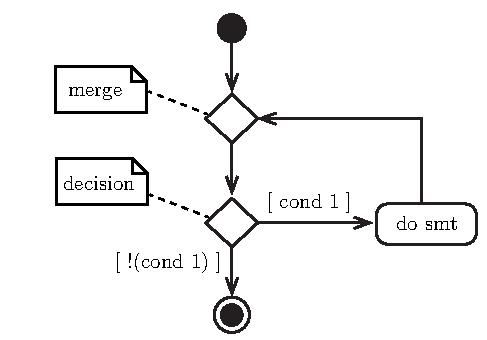
\includegraphics[width=0.50\linewidth]{01_Basics/figures/uml/IterationStatement-00-UML-while.pdf}
% \captionof{figure}{UML \texttt{while} Activity Diagram Representation}
% \label{fig:ch01_Basics_UML_IterationStatement-00-while}
% %~\ref{fig:ch01_Basics_UML_IterationStatement-00-while} 
% %%%%%%%%%%%%%%%%%%%%%%%%%%End figure
% \end{minipage}
% \begin{minipage}{.25\textwidth}
% %%%%%%%%%%%%%%%%%%%%%%%%%%%%%%%%%Begin code
% \begin{lstlisting}[frame=tlrb,numbers=none,mathescape=true,escapechar=\%,columns=flexible]
% some awesome code here
% \end{lstlisting}
% %%%%%%%%%%%%%%%%%%End Code
% \end{minipage}
% \vspace{0.5cm}
% %end minipages


%\begin{enumerate}
%	\item Initialize timer and directions registers
%    \item Specify initial state
%    \item Perform FSM controller
%   \begin{enumerate}
%    	\item Call an output function, which depends on the state
%        \item Delay, which depends on the state
%        \item Call an input function to get the status of the coin sensors
%        \item Change states, which dependes on the state and the input
%    \end{enumerate}
%\end{enumerate}

% \begin{enumerate}
% 	\item Current instruction is finished,
%     \item Eight registers are pushed on the stack,
%     \item LR is set to 0xFFFFFFF9,
%     \item IPSR is set to the interrupt number,
%     \item PC is loaded with the interrupt vector
% \end{enumerate}

% Itemize categoriza poniendo (.) en lugar de números
% \begin{itemize} 
% 	\item I
% 	\item I
% 	\item Y
% 	\item Y
% 	\item Y
% 	\item Y
% 	\item 
% \end{itemize}

% \begin{table}[!h]
% \centering
% \begin{tabular}{|l|l|l|} \hline
% $p$ & bit Field & Interrupt         \\\hline
% $3$ & \bitsRange[31]{29} & Interrupt [$4m+3$]  \\\hline
% $2$ & \bitsRange[23]{21} & Interrupt [$4m+2$]  \\\hline
% $1$ & \bitsRange[15]{13} & Interrupt [$4m+1$]  \\\hline
% $0$ & \bitsRange[7]{5} & Interrupt [$4m$]   \\\hline
% \end{tabular}
% \caption{pasteCaption}
% \label{tab:t_rt_ch04_}
% ~\ref{tab:t_rt_ch04_}
% \end{table}

% Insertar URL
%\url{https://www.osha.gov/Publications/laboratory/OSHAfactsheet-laboratory-safety-noise.pdf}\\
%\href{}{}

% \newcommand{\bitsRange}[2][50]{\texttt{{#1}-{#2}}}
% \newcommand{\CustomHex}[2][0000]{\texttt{0x{#1}.{#2}}}
% \newcommand{\GPIOPort}[1]{\texttt{GPIO\_PORT{#1}}}
% \newcommand{\GPIOPortR}[2][A]{\texttt{GPIO\_PORT{#1}\_{#2}\_R}}
% \newcommand{\GPIOPortHandler}[1]{\texttt{GPIO\_PORT{#1}\_Handler}}
% \newcommand{\HandlerISR}[1]{\texttt{#1\_Handler}}
% \newcommand{\IRQnr}[1]{\texttt{{#1}}}
% \newcommand{\NVICPRI}[1]{\texttt{NVIC\_PRI{#1}\_R}}
% \newcommand{\NVICEN}[1]{\texttt{NVIC\_EN{#1}\_R}}
% \newcommand{\NVICDIS}[1]{\texttt{NVIC\_DIS{#1}\_R}}
% \newcommand{\Ttimer}[2][A]{\texttt{Timer\_{#2}{#1}}}
% \newcommand{\xNrbit}[1]{$#1$-\texttt{bit}}
% \newcommand{\xNrbits}[1]{$#1$-\texttt{bits}}
% \newcommand{\camouflagegreenCellColor}{\cellcolor[rgb]{0.47, 0.53, 0.42}}
% \newcommand{\lavenderCellColor}{\cellcolor[rgb]{0.9, 0.9, 0.98}}
% \newcommand{\volties}[2][0]{$\si{{#1}\volt}_{#2}$}
% \newcommand{\volti}[1]{$\si{{#1}\volt}$}
% \newcommand{\voltiposi}[1]{$+\si{{#1}\volt}$}
% \newcommand{\voltinega}[1]{$-\si{{#1}\volt}$}   \newpage

%%%%%%% ACRONYMS 
\hspace{-1.cm} \large{Akronyme}\\
\begin{acronym}[ABCDEFGHIJK]
%A
\acro{API}{Application Programming Interface} %\ac{API}
\acro{APB}{Advanced Peripheral Bus} %\ac{APB}
%D
\acro{DAE}{Differential-Algebraic Equation}
\acro{DDI}{Differential Dissipativity Inequality}%\ac{DDI} 
\acro{DOF}{Degrees of Freedom}
\acro{DXL}{Rational DOORS Extension Language}%\ac{DXL}
%E
\acro{ES}{Energy Shaping}
%I
\acro{IDA}{Interconnection and Damping Assignment}
\acro{IDA-PBC}{Interconnection and Damping Assignment - Passivity-Based Control}
\acro{IDE}{Integral Dissipation Inequality}%\ac{IDE}
\acro{ISR}{Interrupt Service Routine} %\ac{ISR}
%P
\acro{PBC}{Passivity Based Control}
\acro{PDE}{Partial Differential Equation}
\acro{PFL}{Partial Feedback Linearization}
\acro{pH}{port-Hamiltonian}
%R
\acro{RTOS}{Real Time Operating System} %\ac{RTOS}
%S
\acro{SMC}{Sliding Mode Control}
\acro{SysML}{System Modelling Language} % \ac{UMS}
%U
\acro{UMS}{Underactuated Mechanical System} % \ac{UMS}
\acro{UML}{Unified Modelling Language} % \ac{UMS}
%Z
\acro{ZSD}{Zero-State detectable}
\acro{ZSO}{Zero-State observable}%\ac*{ZSO}
\end{acronym}

%chapter*{\glossarytitlename}
%\addcontentsline{toc}{chapter}{Abbreviations}


% %AQUI TABLA DE ACRÓNIMOS
% \addcontentsline{toc}{chapter}{Abbreviations}
% \begin{acronym}[ABCDEFGHIJK]
% %B
% \acro{BIBO}{Bounded Input Bounded Output}%\ac{BIBO}
% \acro{BP}{Betriebspunkt} %\ac{BP}
% %C
% \acro{CBC}{Cornering Brake Control}%\ac{CBC}
% %D
% \acro{DAP}{Dual Active Pumps} %\ac{DAP}
% \acro{DB}{Driver Braking} %\ac{DB}
% \acro{DGL}{Differential Gleichung} %\ac{DGL}
% \acro{DRP}{Dynamic Rear proportioning} %\ac{DRP}
% %I
% \acro{IBC}{Integrated Braking Control} %\ac{IBC}
% \acro{IDE}{Integrated Development Environment}%\ac{IDE}
% \acro{IRT}{Input rod travel} %\ac{IRT]
% %L
% \acro{LPA}{Low Pressure Accumulator} %\ac{LPA]
% %M
% \acro{MCP}{Master Chamber Pressure} %ac{MCP}
% %N
% \acro{NVH}{Noise Vibration Harshness} %\ac{NVH}
% %P
% \acro{PTS}{Pedal Travel Sensor} %\ac{PTS}
% %R
% \acro{RPO}{Remaining Pressure Optimization}
% %V
% \acro{VSC}{Vehicle Stability Contro} %\ac{VSC}

% \end{acronym}
%%%%%%% END ACRONYMS
%\clearpage

\newpage
%%%%%%% BIBLIOGRAPHY
\bibliographystyle{IEEEtran}
\bibliography{myReferences}
%%%%%%% END BIBLIOGRAPHY
\end{document}
